% --- Configuration ------------------------------------------------------
% add shortcut for github url of this chapter
\def \GITHUB {\GITHUBBASE/02_theory_of_sound_field_synthesis}
% add the fig folders
\graphicspath{%
{\PATH/\CHAPTWO/fig2_01/}%
{\PATH/\CHAPTWO/fig2_02/}%
{\PATH/\CHAPTWO/fig2_03/}%
{\PATH/\CHAPTWO/fig2_04/}%
{\PATH/\CHAPTWO/fig2_05/}%
{\PATH/\CHAPTWO/fig2_06/}%
{\PATH/\CHAPTWO/fig2_07/}%
{\PATH/\CHAPTWO/fig2_08/}%
{\PATH/\CHAPTWO/fig2_09/}%
{\PATH/\CHAPTWO/fig2_10/}%
{\PATH/\CHAPTWO/fig2_11/}%
{\PATH/\CHAPTWO/fig2_12/}%
{\PATH/\CHAPTWO/fig2_13/}%
}


% --- Document -----------------------------------------------------------
\chapter{Theory of Sound Field Synthesis}
\label{cha:sfs}

%\begin{figure}
%    \small
%    \centering
%    \begin{tikzpicture}
    \draw (0,0) node [right] {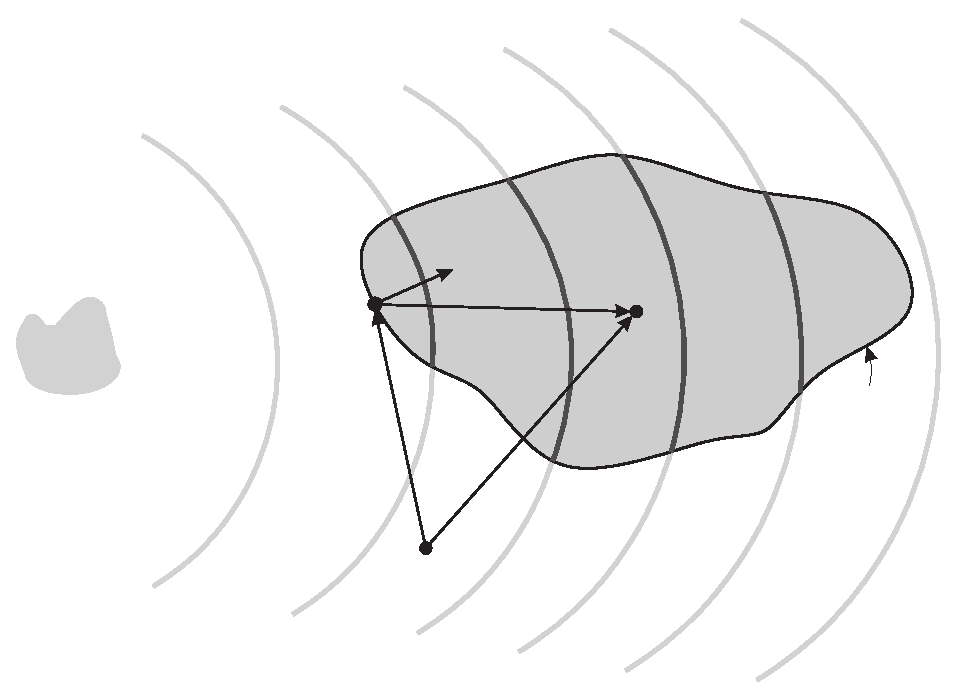
\includegraphics[scale=0.5]{KHint}};
    \draw (0.6,-0.6) node {virtual}; \draw (0.6,-0.9) node {source};
    \draw (6.9,-1.7) node {$S(\x,\omega)$}; \draw (2.84, 0.4) node {$\x_0$};
    \draw (3.9, 0.8) node {$\n$}; \draw (5.55, 0.35) node {$\x$};
    \draw (4.24, 0.0) node {$P(\x,\omega)$}; \draw (5.2, 0.9) node {$V$};
    \draw (7.3,-0.5) node {$\partial V$}; \draw (3.56,-1.9) node {$0$};
\end{tikzpicture}

%    \caption{Illustration of the geometry used to discuss the physical
%        fundamentals of sound field synthesis and the single-layer
%        potential~\protect\eqref{eq:single:layer}.
%        \reproduce{\GITHUB/fig2_01}}
%    \label{fig:KHint}
%\end{figure}

The problem of sound field synthesis can be formulated as
follows.\cite[Small parts of this section are published in][]{Wierstorf2013b}
Assume a volume $V \subset \R^n$
which is free of any sources and sinks,
surrounded by a distribution of monopole sources on its
surface $\partial V$. The pressure $P(\x,\omega)$ at a point $\x \in V$ is then
given by the \emph{single-layer potential}
%
\begin{equation}
    P(\x,\omega) = \oint_{\partial V} D(\x_0,\omega) G(\x-\x_0,\omega) \; \D A(\x_0) \qc
    \eqlabel{single:layer}
\end{equation}
%
where $G(\x-\x_0,\omega)$ denotes the sound propagation of the source at
location $\x_0 \in \partial V$, and $D(\x_0,\omega)$ its weight, usually
referred to as \emph{driving function}. The sources on the surface are called
\emph{secondary sources} in sound field synthesis, analogue to the case of acoustical
scattering problems. The single-layer potential can be derived from the
Kirchhoff-Helmholtz integral.\cite{Williams1999}
The challenge in sound field synthesis is to solve the integral
with respect to $D(\x_0,\omega)$ for
a desired sound field $P = S$ in $V$.
It has unique solutions which Zotter and
Spors\cite{Zotter2013} explicitly
showed for the spherical case and Fazi\cite[][Chap.\,4.3]{Fazi2010} for the
planar case.

In the following the single-layer potential for different
dimensions is discussed. An approach
to formulate the desired sound field $S$ is described and finally it is
shown how to derive the driving function $D$.


%%%%%%%%%%%%%%%%%%%%%%%%%%%%%%%%%%%%%%%%%%%%%%%%%%%%%%%%%%%%%%%%%%%%%%%%%%%%%%%%
\section[Near-Field Compensated Higher Order Ambisonics]{Solution for Special
Geometries: Near-Field Compensated Higher Order Ambisonics and Spectral Division Method}
\label{sec:HOA_SDM}

The integral equation~\eqref{eq:single:layer} states a Fredholm
equation of first kind with a Green's function as kernel. This type of equation
can be solved in a straightforward manner for geometries that have a complete
set of orthogonal basis functions. Then the involved functions are expanded
into the basis functions $\psi_n$ as\cite[Compare][p.\,940]{Morse1981}
%
\begin{equation}
    G(\x-\x_0,\omega) = \sum_{n=1}^N \tilde{G}_n(\omega) \,
        \psi_n^*(\x_0) \psi_n(\x)
    \label{eq:G_expansion}
\end{equation}
%
\begin{equation}
    D(\x_0,\omega) = \sum_{n=1}^N \tilde{D}_n(\omega) \,
        \psi_n(\x_0)
    \label{eq:D_expansion}
\end{equation}
%
\begin{equation}
    S(\x,\omega) = \sum_{n=1}^N \tilde{S}_n(\omega) \,
        \psi_n(\x) \qc
    \label{eq:S_expansion}
\end{equation}
%
where $\tilde{G}_n, \tilde{D}_n, \tilde{S}_n$ denote the series expansion
coefficients and \linebreak $\langle\psi_n, \psi_{n'}\rangle = 0$ for $n \ne n'$.
%$\psi_n^*$ is the complex conjugate of $\psi_n$ for a symmetrical kernel.
Introducing these three equations
into~\eqref{eq:single:layer} one gets
%
\begin{equation}
    \tilde{D}_n(\omega) = \frac{\tilde{S}_n(\omega)}{\tilde{G}_n(\omega)} \qp
    \label{eq:D_HOA}
\end{equation}
%
This means that the Fredholm equation~\eqref{eq:single:layer}
states a convolution. For geometries where
the required orthogonal basis functions exist, \eqref{eq:D_HOA} follows directly via
the convolution theorem.\cite[Compare][p.\,1013]{Arfken2005}
Due to the division of the desired sound field by the spectrum of the
Green's function this kind
of approach has been named \acf{SDM}.\cite{Ahrens2010a}
For circular and spherical geometries the term \acf{NFC-HOA} is more common due
to the corresponding basis functions. ``Near-field compensated'' highlights the
usage of point sources as secondary sources in contrast to Ambisonics and
\acf{HOA} that assume plane waves as secondary sources.

The challenge is to find a set of basis functions for a given geometry. In
the following paragraphs three simple geometries and their widely known sets of basis
functions will be discussed.

%--%--%--%--%--%--%--%--%--%--%--%--%--%--%--%--%--%--%--%--%--%--%--%--%--%--%-
\subsection{Spherical Geometries}
\label{sec:spherical_geometries}

The spherical
harmonic functions constitute a basis for a spherical secondary source distribution
in $\R^3$ and can be defined as\cite[][(12.153), $\sin\theta$ is used here instead
of $\cos\theta$ due to the use of
another coordinate system, compare Figure\,2.1 from Gumerov and Duraiswami and
Figure\,\ref{fig:coordinate_system} in this thesis.]{Gumerov2004}
%
\begin{gather}
    Y_n^m(\theta,\phi) = (-1)^m \sqrt{\frac{(2n+1)(n-|m|)!}{4\PI(n+|m|)!}}
    P_n^{|m|}(\sin\theta) \E^{\I m\phi} \qc
    \label{eq:Y} \\
    n = 0,1,2,... \;\;\;\;\;\; m = -n,...,n
    \notag
\end{gather}
%
where $P_n^{|m|}$ are the associated Legendre functions. Note that this function
may also be defined in a slightly different way, omitting the $(-1)^m$ factor,
see for example Williams.\cite[][(6.20)]{Williams1999}

The complex conjugate of $Y_n^m$ is given by negating the degree $m$ as
%
\begin{equation}
    Y_n^m(\theta,\phi)^* = Y_n^{-m}(\theta,\phi) \qp
    \label{eq:Y_complex_conjugate}
\end{equation}
%

For a spherical secondary source distribution with a radius of $R_0$
the sound field can be calculated by a convolution along the surface.
The driving function is then given by a simple division
as\cite[][(3.21)]{Ahrens2012}. The $\frac{1}{2\PI}$ term is wrong in
(3.21) and omitted here, compare the
\url{errata}{http://www.soundfieldsynthesis.org/errata/} and \cite[][(24)]{Schultz2014}.
%
\begin{multline}
    D_\text{spherical}(\theta_0,\phi_0,\omega) = \\ 
    \frac{1}{R_0^{\,2}}
    \sum_{n=0}^\infty \sum_{m=-n}^n \sqrt{\frac{2n+1}{4\PI}}
    \frac{\breve{S}_n^m(\theta_\text{s},\phi_\text{s},r_\text{s},\omega)}
    {\breve{G}_n^0(\frac{\PI}{2},0,\omega)} Y_n^m(\theta_0,\phi_0) \qc
    \label{eq:D_spherical}
\end{multline}
%
where $\breve{S}_n^m$ denote the spherical expansion
coefficients of the source model, $\theta_\text{s}$ and
$\phi_\text{s}$ its directional dependency, and $\breve{G}_n^0$
the spherical expansion coefficients of a
secondary point source that is located at the north pole of the sphere with $\x_0 =
(0,0,R_0)$ and is given as\cite[][(25)]{Schultz2014}
%
\begin{equation}
    \breve{G}_n^0(\tfrac{\PI}{2},0,\omega) =
    -\I\omegac \sqrt{\frac{2n+1}{4\PI}} \h{n}{2}\left(\omegac R_0\right) \qc
    \label{eq:G_spherical}
\end{equation}
where $\h{n}{2}$ describes the spherical Hankel function of $n$-th order and
second kind.


%--%--%--%--%--%--%--%--%--%--%--%--%--%--%--%--%--%--%--%--%--%--%--%--%--%--%-
\subsection{Circular Geometries}
\label{sec:circular_geometries}

The following functions build a basis in $\R^2$ for a circular secondary source
distribution\cite{Williams1999}
%
\begin{equation}
    \Phi_m(\phi) = \E^{\I m\phi} \qp
    \label{eq:circular_harmonics}
\end{equation}
%
The complex conjugate of $\Phi_m$ is given by negating the degree $m$ as
%
\begin{equation}
    \Phi_m(\phi)^* = \Phi_{-m}(\phi) \qp
    \label{eq:Phi_complex_conjugate}
\end{equation}
%

For a circular secondary source distribution with a radius of $R_0$ the
driving function can
be calculated by a convolution along the surface of the circle as explicitly
shown by Ahrens\cite{Ahrens2009c} and is then given as
%
\begin{equation}
    D_\text{circular}(\phi_0,\omega) = \frac{1}{2\PI R_0} \sum_{m=-\infty}^\infty 
    \frac{\breve{S}_m(\phi_\text{s},r_\text{s},\omega)}{\breve{G}_m(0,\omega)} \,
    \Phi_m(\phi_0) \qc
    \label{eq:D_circular}
\end{equation}
%
where $\breve{S}_m$ denotes the circular expansion coefficients for
the source model, $\phi_\text{s}$ its directional dependency, and $\breve{G}_m$
the circular expansion coefficients for a secondary line source with
%
\begin{equation}
    \breve{G}_m(0,\omega) = -\frac{\I}{4} \H{m}{2}\left(\omegac R_0\right) \qc
    \label{eq:G_circular}
\end{equation}
%
where $\H{m}{2}$ describes the Hankel function of $m$-th order and second kind.


%--%--%--%--%--%--%--%--%--%--%--%--%--%--%--%--%--%--%--%--%--%--%--%--%--%--%-
\subsection{Planar Geometries}
\label{sec:planar_geometries}

The basis functions for a planar secondary source distribution
located on the $xz$-plane in $\R^3$ are given as
%
\begin{equation}
    \Lambda(k_x,k_z,x,z) = \E^{-\I(k_x x + k_z z)} \qc
    \label{eq:planar_harmonics}
\end{equation}
%
where $k_x$, $k_z$ are entries in the wave vector $\k$ with $k^2 =
(\omegac)^2$.
The complex conjugate is given by negating $k_x$ and $k_z$ as
%
\begin{equation}
    \Lambda(k_x,k_z,x,z)^* = \Lambda(-k_x,-k_z,x,z) \qp
\end{equation}
%

For an infinitely long secondary source distribution located on the
$xz$-plane the driving function can be calculated by a two-dimensional
convolution along the plane as\cite[][(3.65)]{Ahrens2012}
%
\begin{equation}
    D_\text{planar}(x_0,\omega) = \frac{1}{4\PI^2} \iint_{-\infty}^\infty
    \frac{\breve{S}(k_x,y_\text{s},k_z,\omega)}{\breve{G}(k_x,0,k_z,\omega)}
    \Lambda(k_x,x_0,k_z,z_0) \, \D{k_x} \D{k_z} \qc
    \label{eq:D_planar}
\end{equation}
%
where $\breve{S}$ denotes the planar expansion coefficients for the
source model, $y_\text{s}$ its positional dependency, and $\breve{G}$ the planar
expansion coefficients of a secondary point source with\cite[][(65)]{Schultz2014}
%
\begin{equation}
    \breve{G}(k_x,0,k_z,\omega) = -\frac{\I}{2}
    \frac{1}{\sqrt{(\omegac)^2-k_x^2-k_z^2}}
    \qc
    \label{G_planar}
\end{equation}
%
for $(\omegac)^2 > (k_x^2+k_z^2)$.

For the planar and the following linear geometries the Fredholm equation is
solved for a non compact space $V$, which leads to an infinite and
non-denumerable number of basis functions as
opposed to the denumerable case for compact spaces.\cite{Schultz2014}


%--%--%--%--%--%--%--%--%--%--%--%--%--%--%--%--%--%--%--%--%--%--%--%--%--%--%-
\subsection{Linear Geometries}
\label{sec:linear_geometries}

The basis functions for a linear secondary source distribution
located on the $x$-axis are given as
%
\begin{equation}
    \chi(k_x,x) = \E^{-\I k_x x} \qp
    \label{eq:linear_harmonics}
\end{equation}
%
The complex conjugate is given by negating $k_x$ as
%
\begin{equation}
    \chi(k_x,x)^* = \chi(-k_x,x) \qp
\end{equation}
%

For an infinitely long secondary source distribution located on the $x$-axis the
driving function for $\R^2$ can be calculated by a convolution along this axis
as\cite[Compare (3.73) in][]{Ahrens2012}
%
\begin{equation}
    D_\text{linear}(x_0,\omega) = \frac{1}{2\PI} \int_{-\infty}^\infty
    \frac{\breve{S}(k_x,y_\text{s},\omega)}{\breve{G}(k_x,0,\omega)}
    \chi(k_x,x_0) \, \D{k_x} \qc
    \label{eq:D_linear}
\end{equation}
%
where $\breve{S}$ denotes the linear expansion coefficients for the
source model, $y_\text{s}$, $z_\text{s}$ its positional dependency,
and $\breve{G}$ the linear expansion coefficients of a secondary line source with
%
\begin{equation}
    \breve{G}(k_x,0,\omega) = -\frac{\I}{2} \frac{1}{\sqrt{(\omegac)^2-k_x^2}}
    \qc
    \label{eq:G_linear}
\end{equation}
%
for $0<|k_x|<|\omegac|$.


%%%%%%%%%%%%%%%%%%%%%%%%%%%%%%%%%%%%%%%%%%%%%%%%%%%%%%%%%%%%%%%%%%%%%%%%%%%%%%%%%
\section[Wave Field Synthesis]{High Frequency Approximation: Wave Field Synthesis}
\label{sec:WFS}

The single-layer potential~\eqref{eq:single:layer} satisfies the homogeneous
Helmholtz equation
\index{Helmholtz equation}
both in the interior and exterior regions $V$ and $V^*
\defeq \R^n \setminus (V \cup \partial V)$.  If $D(\x_0,\omega)$ is
continuous, the pressure $P(\x,\omega)$ is continuous when approaching the
surface $\partial V$ from the inside and outside.  Due to the presence of the
secondary sources at the surface $\partial V$, the gradient of $P(\x,\omega)$ is
discontinuous when approaching the surface.
The strength of the secondary sources is then given by the differences of the
gradients approaching $\partial V$ from both sides
as\cite[Compare][]{Fazi2013}
%
\begin{equation}
    D(\x_0,\omega) = \partial_\n
    P(\x_0,\omega) + \partial_{-\n} P(\x_0,\omega)\qc
    \label{eq:D_gradient}
\end{equation}
%
where
$\partial_\n\!\defeq\!\langle\nabla,\n\rangle$ is the directional gradient
in direction $\n$ -- see Figure\,\ref{fig:KHint}.
Due to the symmetry of the problem the solution for an infinite planar
boundary $\partial V$ is given as 
%
\begin{equation}
    D(\x_0,\omega) = -2 \partial_\n S(\x_0,\omega)\qc
    \label{eq:D_wfs}
\end{equation}
%
where the pressure in the outside region is the mirrored interior pressure given by the
source model $S(\x,\omega)$ for $\x \in V$.  The
integral equation resulting from introducing~\eqref{eq:D_wfs}
into~\eqref{eq:single:layer} for a planar boundary $\partial V$ is known as
{\em Rayleigh's first integral equation}. This solution is identical
to the explicit solution for planar geometries~\eqref{eq:D_planar} in $\R^3$ and for
linear geometries~\eqref{eq:D_linear} in $\R^2$.

A solution of~\eqref{eq:D_gradient} for  arbitrary boundaries can be
found by applying the \emph{Kirchhoff} or \emph{physical optics
approximation}.\cite[See][p.\,53--54]{Colton1983}
\index{Kirchhoff approximation}
In acoustics this is also known as \emph{determining the visible elements} for
the high frequency boundary element
method.\cite[E.g.][]{Herrin2003}
Here, it is assumed that a
bent surface can be approximated by a set of small planar surfaces for
which~\eqref{eq:D_wfs} holds locally.  In general, this will be the case if the
wave length is much smaller than the size of a planar surface patch and the
position of the listener is far away from the secondary
sources.\cite[Compare the two assumptions in][made before
(15), which lead to the derivation of the same window function in a more explicit way.]{Spors2013}
Additionally, only one part of the surface is active: the area that is
illuminated from the incident field of the source model.
With this approximation
also non-convex secondary
source distributions can be used with
WFS -- compare
Figure\,\ref{fig:concave_array}.\cite[See the appendix
in][]{Lax1947}
This was neglected in most of the literature so far, which postulates
convex secondary source
distributions.\cite[E.g.][]{Spors2008}


%\begin{figure}
%    \small
%    \centering
%    % GNUPLOT: LaTeX picture with Postscript
\begingroup
  \makeatletter
  \providecommand\color[2][]{%
    \GenericError{(gnuplot) \space\space\space\@spaces}{%
      Package color not loaded in conjunction with
      terminal option `colourtext'%
    }{See the gnuplot documentation for explanation.%
    }{Either use 'blacktext' in gnuplot or load the package
      color.sty in LaTeX.}%
    \renewcommand\color[2][]{}%
  }%
  \providecommand\includegraphics[2][]{%
    \GenericError{(gnuplot) \space\space\space\@spaces}{%
      Package graphicx or graphics not loaded%
    }{See the gnuplot documentation for explanation.%
    }{The gnuplot epslatex terminal needs graphicx.sty or graphics.sty.}%
    \renewcommand\includegraphics[2][]{}%
  }%
  \providecommand\rotatebox[2]{#2}%
  \@ifundefined{ifGPcolor}{%
    \newif\ifGPcolor
    \GPcolortrue
  }{}%
  \@ifundefined{ifGPblacktext}{%
    \newif\ifGPblacktext
    \GPblacktextfalse
  }{}%
  % define a \g@addto@macro without @ in the name:
  \let\gplgaddtomacro\g@addto@macro
  % define empty templates for all commands taking text:
  \gdef\gplbacktext{}%
  \gdef\gplfronttext{}%
  \makeatother
  \ifGPblacktext
    % no textcolor at all
    \def\colorrgb#1{}%
    \def\colorgray#1{}%
  \else
    % gray or color?
    \ifGPcolor
      \def\colorrgb#1{\color[rgb]{#1}}%
      \def\colorgray#1{\color[gray]{#1}}%
      \expandafter\def\csname LTw\endcsname{\color{white}}%
      \expandafter\def\csname LTb\endcsname{\color{black}}%
      \expandafter\def\csname LTa\endcsname{\color{black}}%
      \expandafter\def\csname LT0\endcsname{\color[rgb]{1,0,0}}%
      \expandafter\def\csname LT1\endcsname{\color[rgb]{0,1,0}}%
      \expandafter\def\csname LT2\endcsname{\color[rgb]{0,0,1}}%
      \expandafter\def\csname LT3\endcsname{\color[rgb]{1,0,1}}%
      \expandafter\def\csname LT4\endcsname{\color[rgb]{0,1,1}}%
      \expandafter\def\csname LT5\endcsname{\color[rgb]{1,1,0}}%
      \expandafter\def\csname LT6\endcsname{\color[rgb]{0,0,0}}%
      \expandafter\def\csname LT7\endcsname{\color[rgb]{1,0.3,0}}%
      \expandafter\def\csname LT8\endcsname{\color[rgb]{0.5,0.5,0.5}}%
    \else
      % gray
      \def\colorrgb#1{\color{black}}%
      \def\colorgray#1{\color[gray]{#1}}%
      \expandafter\def\csname LTw\endcsname{\color{white}}%
      \expandafter\def\csname LTb\endcsname{\color{black}}%
      \expandafter\def\csname LTa\endcsname{\color{black}}%
      \expandafter\def\csname LT0\endcsname{\color{black}}%
      \expandafter\def\csname LT1\endcsname{\color{black}}%
      \expandafter\def\csname LT2\endcsname{\color{black}}%
      \expandafter\def\csname LT3\endcsname{\color{black}}%
      \expandafter\def\csname LT4\endcsname{\color{black}}%
      \expandafter\def\csname LT5\endcsname{\color{black}}%
      \expandafter\def\csname LT6\endcsname{\color{black}}%
      \expandafter\def\csname LT7\endcsname{\color{black}}%
      \expandafter\def\csname LT8\endcsname{\color{black}}%
    \fi
  \fi
  \setlength{\unitlength}{0.0500bp}%
  \begin{picture}(5668.00,2834.00)%
    \gplgaddtomacro\gplbacktext{%
      \colorrgb{0.50,0.50,0.50}%
      \put(1025,220){\makebox(0,0)[r]{\strut{}$-10$}}%
      \colorrgb{0.50,0.50,0.50}%
      \put(1025,612){\makebox(0,0)[r]{\strut{}$-8$}}%
      \colorrgb{0.50,0.50,0.50}%
      \put(1025,1003){\makebox(0,0)[r]{\strut{}$-6$}}%
      \colorrgb{0.50,0.50,0.50}%
      \put(1025,1395){\makebox(0,0)[r]{\strut{}$-4$}}%
      \colorrgb{0.50,0.50,0.50}%
      \put(1025,1786){\makebox(0,0)[r]{\strut{}$-2$}}%
      \colorrgb{0.50,0.50,0.50}%
      \put(1025,2178){\makebox(0,0)[r]{\strut{}$0$}}%
      \colorrgb{0.50,0.50,0.50}%
      \put(1025,2569){\makebox(0,0)[r]{\strut{}$2$}}%
      \colorrgb{0.50,0.50,0.50}%
      \put(1334,63){\makebox(0,0){\strut{}$-8$}}%
      \colorrgb{0.50,0.50,0.50}%
      \put(1725,63){\makebox(0,0){\strut{}$-6$}}%
      \colorrgb{0.50,0.50,0.50}%
      \put(2117,63){\makebox(0,0){\strut{}$-4$}}%
      \colorrgb{0.50,0.50,0.50}%
      \put(2508,63){\makebox(0,0){\strut{}$-2$}}%
      \colorrgb{0.50,0.50,0.50}%
      \put(2900,63){\makebox(0,0){\strut{}$0$}}%
      \colorrgb{0.50,0.50,0.50}%
      \put(3291,63){\makebox(0,0){\strut{}$2$}}%
      \colorrgb{0.50,0.50,0.50}%
      \put(3682,63){\makebox(0,0){\strut{}$4$}}%
      \colorrgb{0.50,0.50,0.50}%
      \put(4074,63){\makebox(0,0){\strut{}$6$}}%
      \colorrgb{0.50,0.50,0.50}%
      \put(4465,63){\makebox(0,0){\strut{}$8$}}%
      \csname LTb\endcsname%
      \put(519,1394){\rotatebox{-270}{\makebox(0,0){\strut{}$y$ / m}}}%
      \put(2899,-157){\makebox(0,0){\strut{}$x$ / m}}%
    }%
    \gplgaddtomacro\gplfronttext{%
    }%
    \gplbacktext
    \put(0,0){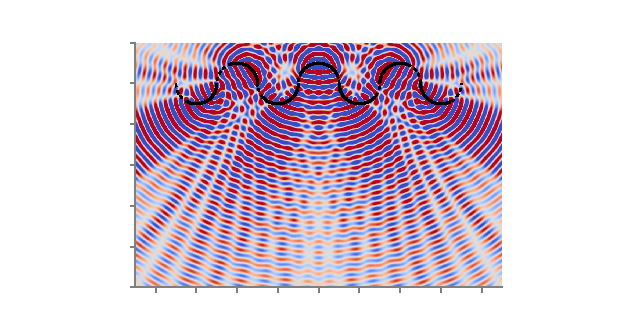
\includegraphics{concave_array}}%
    \gplfronttext
  \end{picture}%
\endgroup

%    \caption{Sound pressure of a point source synthesized with
%    \ac{WFS}~\protect\eqref{eq:D:wfs:ps:2.5D}. The secondary source
%        distribution is shown in black, whereby inactive sources are marked with a
%        dashed line. Parameters: $\xs = (0,2.5,0)$\,m,
%        $\xref = (0,-3,0)$\,m, $f = 700$\,Hz.
%        \reproduce{\GITHUB/fig2_02}}
%    \label{fig:concave_array}
%\end{figure}

The outlined approximation can be formulated by
introducing a window function $w(\x_0)$ for the selection of the active
secondary sources into~\eqref{eq:D_wfs} as
%
\begin{equation}
    P(\x,\omega) \approx \oint_{\partial V} \!\!  G(\x|\x_0,\omega) \,
    \underbrace{-2 w(\x_0) \partial_\n S(\x_0,\omega)}_{D(\x_0,\omega)} \; \D
    A(\x_0) \qp
    \label{eq:P_wfs}
\end{equation}
%

One of the advantages of the applied approximation is that due to its local
character the solution of the driving function~\eqref{eq:D_wfs} does not depend on
the geometry of the secondary sources. This dependency applies to the direct
solutions presented in Section\,\ref{sec:HOA_SDM}.


%%%%%%%%%%%%%%%%%%%%%%%%%%%%%%%%%%%%%%%%%%%%%%%%%%%%%%%%%%%%%%%%%%%%%%%%%%%%%%%%%
\section{Sound Field Dimensionality}
\label{sec:sound_field_dimensionality}
%
The single-layer potential~\eqref{eq:single:layer} is valid for all $V
\subset \R^n$. Consequentially, for practical applications a two-dimensional
(\twoD) as well as a three-dimensional (\threeD) synthesis is possible.
Two-dimensional is not referring to a synthesis in a plane only, but describes a setup
that is independent of one dimension. For example, an infinite cylinder is
independent of the dimension along its axis. The same is true
for secondary source distributions in \twoD synthesis. They exhibit
line source characteristics and are aligned in parallel to
the independent dimension. Typical arrangements of such secondary sources are
a circular or a linear setup.

The characteristics of the secondary
sources limit the set of possible sources which can be synthesized. For example,
when using a \twoD secondary source setup it is not possible to synthesize the
amplitude decay of a point source.

For a \threeD synthesis the involved secondary sources depend on all dimensions
and exhibit point source characteristics. In this scenario
classical secondary sources setups would be a sphere or a plane.

%--%--%--%--%--%--%--%--%--%--%--%--%--%--%--%--%--%--%--%--%--%--%--%--%--%--%-
\subsection{\twohalfD Synthesis}
\label{sec:25d_synthesis}
%
%\begin{figure}
%    \centering
%    \small
%    \begin{tikzpicture}
%        \draw (0,0)       node {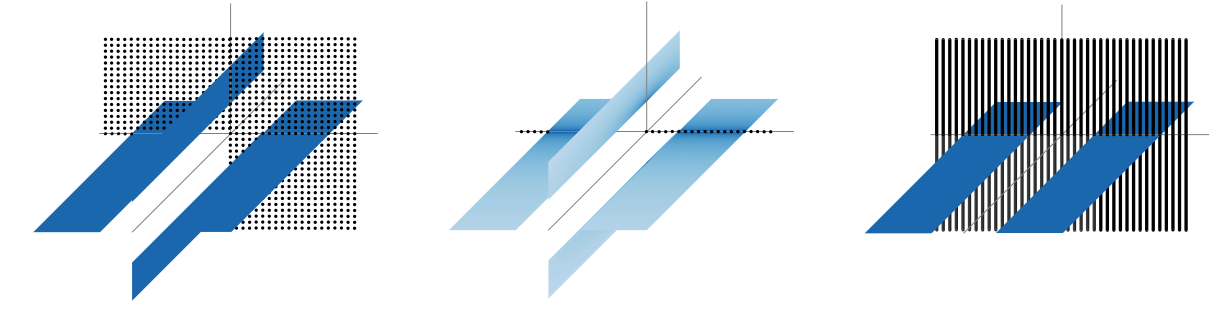
\includegraphics[width=.8\columnwidth]{sound_field_dimensionality}};
%        \draw (-0.75,1.2) node {\twohalfD};
%        \draw (-3.75,1.2) node {\threeD};
%        \draw (2.05,1.2)  node {\twoD};
%    \end{tikzpicture}
%    \caption{Sound pressure in decibel for secondary source distributions with different
%    dimensionality all driven by the same signals. The sound pressure is color
%    coded, lighter color corresponds to lower pressure.
%    In the \threeD case a planar distribution of point sources is applied,
%    in the \twohalfD case a linear distribution of point sources, and in the \twoD
%    case a linear distribution of line sources.
%    \reproduce{\GITHUB/fig2_03}}
%    \label{fig:sound_field_dimensionality}
%\end{figure}
%
In practice, the most common setups of secondary sources are \twoD setups,
employing cabinet loudspeakers. A cabinet loudspeaker does not show the characteristics
of a line source, but of a point source. This dimensionality mismatch prevents perfect
synthesis within the desired plane. The combination of a \twoD secondary source
setup with secondary
sources that exhibit \threeD characteristics has led to naming such
configurations
\emph{\twohalfD synthesis}.\cite{Start1997} Such scenarios
are associated with a wrong amplitude decay due to the inherent mismatch of secondary
sources as is highlighted in Figure\,\ref{fig:sound_field_dimensionality}.
In general, the amplitude is only correct at a given reference point
$\x_\text{ref}$.

For a circular secondary source distribution with point source characteristic
the \twohalfD driving function
can be derived by introducing expansion coefficients for the spherical case
into the driving function~\eqref{eq:D_circular}. The equation is than solved
for $\theta = 0\degree$ and $r_\text{ref} = 0$. This
results in a \twohalfD driving function given in
Ahrens\cite[][(3.49)]{Ahrens2012} as
%
\begin{equation}
    D_{\text{circular},\twohalfD}(\phi_0,\omega) = \frac{1}{2\PI R_0} \sum_{m=-\infty}^\infty
    \frac{\breve{S}_{|m|}^m (\frac{\PI}{2},\phi_\text{s},r_\text{s},\omega)}{\breve{G}_{|m|}^m
    (\frac{\PI}{2},0,\omega)}
    \Phi_m(\phi_0) \qp
    \label{eq:D_circular_25D}
\end{equation}
%

For a linear secondary source distribution with point source characteristics the
\twohalfD driving function is derived by introducing the
linear expansion coefficients for a monopole
source~\eqref{eq:point_source_linear} into the driving
function~\eqref{eq:D_linear} and solving the equation for $y = y_\text{ref}$ and
$z = 0$. This results in a \twohalfD driving function given
as\cite[][(3.77)]{Ahrens2012}
%
\begin{equation}
    D_{\text{linear},\twohalfD}(x_0,\omega) = \frac{1}{2\PI} \int_{-\infty}^\infty
    \frac{\breve{S}(k_x,y_\text{ref},0,\omega)}
    {\breve{G}(k_x,y_\text{ref},0,\omega)} \chi(k_x,x_0) \, \D{k_x} \qp
    \label{eq:D_linear_25D}
\end{equation}
%

A driving function for the \twohalfD situation in the context of \ac{WFS}
and arbitrary \twoD geometries of the secondary source distribution
can be achieved by applying the
far-field approximation\cite[][(4.23)]{Williams1999}
$\H{0}{2}(\zeta) \approx \sqrt{\frac{2\I}{\PI \zeta}}
\E^{-\I\zeta}$ for $\zeta \gg 1$ to the \twoD Green's function.
Using this the
following relationship between the \twoD and \threeD
Green's functions can be established.
%
\begin{multline} 
    \underbrace{
    -\frac{\I}{4} \;\H{0}{2}\left(\omegac |\x-\x_0|\right)
    }_{G_\twoD(\x-\x_0,\omega)}
    \approx
    \sqrt{2\PI \frac{c}{\I\omega} |\x-\x_0|} \;
    \underbrace{
        \frac{1}{4 \PI} \frac{\E^{-\I\omegac|\x-\x_0|}}{|\x-\x_0|}
    }_{G_\threeD(\x-\x_0,\omega)} \qc
    \label{eq:25D_approximation}
\end{multline}
%
where $\H{0}{2}$ denotes the Hankel function of second kind and zeroth
order.
Inserting this approximation into the single-layer potential for the \twoD
case results in
%
\begin{equation}
    P(\x,\omega) = \oint_S \sqrt{2\PI \frac{c}{\I\omega} |\x-\x_0|} \;
    D(\x_0,\omega) G_\threeD(\x-\x0,\omega) \, \D A(\x_0) \qp
    \label{eq:single:layer_25D}
\end{equation}
%
If the amplitude correction is further restricted to one reference point
$\x_\text{ref}$, the \twohalfD driving function for \ac{WFS} can be formulated
as
%
\begin{equation}
    D_\twohalfD(\x_0,\omega) = \underbrace{\sqrt{2\PI |\x_\text{ref}-\x_0|}}_{g_0}
    \sqrt{\frac{c}{\I\omega}} \,
    D(\x_0,\omega) \qc
    \label{eq:D25D_wfs}
\end{equation}
%
where $g_0$ is independent of $\x$.

\newpage

%%%%%%%%%%%%%%%%%%%%%%%%%%%%%%%%%%%%%%%%%%%%%%%%%%%%%%%%%%%%%%%%%%%%%%%%%%%%%%%%%
\section{Model-Based Rendering}
\label{sec:model_based_rendering}
%
Knowing the pressure field of the desired source $S(\x,\omega)$ is required
in order to derive the driving signal for the secondary source distribution.
It can either be measured, i.e.~recorded, or modeled. While the former is known as
{\em data-based rendering},
the latter is known as {\em model-based rendering}.
For data-based rendering, the problem of how to capture a complete sound field
still has to be solved. Avni et al. discuss some influences of the
recording limitations on the perception of the reproduced sound field.\cite{Avni2013}
This thesis focusses on the perception of the synthesis part. Therefore it
will consider only model-based rendering.

Frequently applied models in model-based rendering are plane waves, point
sources, or sources with a prescribed complex directivity.
In the following the models used within the Sound Field Synthesis
Toolbox are presented.
%
%----%----%----%----%----%----%----%----%----%----%----%----%----%----%----%----
\paragraph{Plane Wave}
\label{sec:plane_wave}
%
The source model for a plane wave is given
as\cite[][p.\,21, (2.24). Williams defines the Fourier transform with transposed
signs as $F(\omega) = \int f(t) \E^{\I\omega t}$. This leads also to changed signs
in his definitions of the Green's functions and field expansions.]{Williams1999}
%
%\begin{figure}
%    \centering
%    \ft
%    % GNUPLOT: LaTeX picture with Postscript
\begingroup
  \makeatletter
  \providecommand\color[2][]{%
    \GenericError{(gnuplot) \space\space\space\@spaces}{%
      Package color not loaded in conjunction with
      terminal option `colourtext'%
    }{See the gnuplot documentation for explanation.%
    }{Either use 'blacktext' in gnuplot or load the package
      color.sty in LaTeX.}%
    \renewcommand\color[2][]{}%
  }%
  \providecommand\includegraphics[2][]{%
    \GenericError{(gnuplot) \space\space\space\@spaces}{%
      Package graphicx or graphics not loaded%
    }{See the gnuplot documentation for explanation.%
    }{The gnuplot epslatex terminal needs graphicx.sty or graphics.sty.}%
    \renewcommand\includegraphics[2][]{}%
  }%
  \providecommand\rotatebox[2]{#2}%
  \@ifundefined{ifGPcolor}{%
    \newif\ifGPcolor
    \GPcolortrue
  }{}%
  \@ifundefined{ifGPblacktext}{%
    \newif\ifGPblacktext
    \GPblacktextfalse
  }{}%
  % define a \g@addto@macro without @ in the name:
  \let\gplgaddtomacro\g@addto@macro
  % define empty templates for all commands taking text:
  \gdef\gplbacktext{}%
  \gdef\gplfronttext{}%
  \makeatother
  \ifGPblacktext
    % no textcolor at all
    \def\colorrgb#1{}%
    \def\colorgray#1{}%
  \else
    % gray or color?
    \ifGPcolor
      \def\colorrgb#1{\color[rgb]{#1}}%
      \def\colorgray#1{\color[gray]{#1}}%
      \expandafter\def\csname LTw\endcsname{\color{white}}%
      \expandafter\def\csname LTb\endcsname{\color{black}}%
      \expandafter\def\csname LTa\endcsname{\color{black}}%
      \expandafter\def\csname LT0\endcsname{\color[rgb]{1,0,0}}%
      \expandafter\def\csname LT1\endcsname{\color[rgb]{0,1,0}}%
      \expandafter\def\csname LT2\endcsname{\color[rgb]{0,0,1}}%
      \expandafter\def\csname LT3\endcsname{\color[rgb]{1,0,1}}%
      \expandafter\def\csname LT4\endcsname{\color[rgb]{0,1,1}}%
      \expandafter\def\csname LT5\endcsname{\color[rgb]{1,1,0}}%
      \expandafter\def\csname LT6\endcsname{\color[rgb]{0,0,0}}%
      \expandafter\def\csname LT7\endcsname{\color[rgb]{1,0.3,0}}%
      \expandafter\def\csname LT8\endcsname{\color[rgb]{0.5,0.5,0.5}}%
    \else
      % gray
      \def\colorrgb#1{\color{black}}%
      \def\colorgray#1{\color[gray]{#1}}%
      \expandafter\def\csname LTw\endcsname{\color{white}}%
      \expandafter\def\csname LTb\endcsname{\color{black}}%
      \expandafter\def\csname LTa\endcsname{\color{black}}%
      \expandafter\def\csname LT0\endcsname{\color{black}}%
      \expandafter\def\csname LT1\endcsname{\color{black}}%
      \expandafter\def\csname LT2\endcsname{\color{black}}%
      \expandafter\def\csname LT3\endcsname{\color{black}}%
      \expandafter\def\csname LT4\endcsname{\color{black}}%
      \expandafter\def\csname LT5\endcsname{\color{black}}%
      \expandafter\def\csname LT6\endcsname{\color{black}}%
      \expandafter\def\csname LT7\endcsname{\color{black}}%
      \expandafter\def\csname LT8\endcsname{\color{black}}%
    \fi
  \fi
  \setlength{\unitlength}{0.0500bp}%
  \begin{picture}(2834.00,2834.00)%
    \gplgaddtomacro\gplbacktext{%
      \colorrgb{0.50,0.50,0.50}%
      \put(550,887){\makebox(0,0)[r]{\strut{}$-1$}}%
      \colorrgb{0.50,0.50,0.50}%
      \put(550,1395){\makebox(0,0)[r]{\strut{}$0$}}%
      \colorrgb{0.50,0.50,0.50}%
      \put(550,1902){\makebox(0,0)[r]{\strut{}$1$}}%
      \colorrgb{0.50,0.50,0.50}%
      \put(1043,350){\makebox(0,0){\strut{}$-1$}}%
      \colorrgb{0.50,0.50,0.50}%
      \put(1550,350){\makebox(0,0){\strut{}$0$}}%
      \colorrgb{0.50,0.50,0.50}%
      \put(2057,350){\makebox(0,0){\strut{}$1$}}%
      \csname LTb\endcsname%
      \put(176,1394){\rotatebox{-270}{\makebox(0,0){\strut{}$y$ / m}}}%
      \put(1550,130){\makebox(0,0){\strut{}$x$ / m}}%
    }%
    \gplgaddtomacro\gplfronttext{%
    }%
    \gplbacktext
    \put(0,0){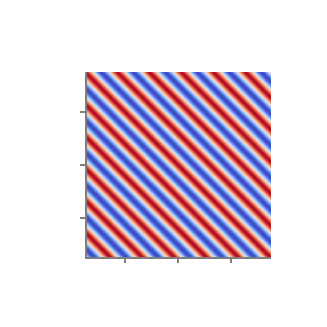
\includegraphics{sound_field_plane_wave}}%
    \gplfronttext
  \end{picture}%
\endgroup

%    \caption{Sound pressure for a monochromatic plane
%        wave~\eqref{eq:S:pw} going into the
%        direction $(1,1,0)$. Parameters: $f = 800$\,Hz.
%        \reproduce{\GITHUB/fig2_04}}
%\end{figure}
%
\begin{equation} 
    S(\x,\omega) = A(\omega) \E^{-\I\omegac \n_k \x}
    \qc
    \eqlabel{S:pw}
\end{equation}
%
where $A(\omega)$ denotes the frequency spectrum of the source
and $\n_k$ a unit vector pointing into the direction of
the plane wave.

Transformed in the temporal domain this becomes
%
\begin{equation}
    s(\x,t) = a(t) * \deltafunc{t -\frac{\n_k \x}{c}}
    \qc
    \eqlabel{s:pw}
\end{equation}
where $a(t)$ is the Fourier transformation of the frequency spectrum $A(\omega)$.

The expansion coefficients for spherical basis functions are given
as\cite[][(2.38)]{Ahrens2012}
%
\begin{equation}
    \breve{S}_n^m(\theta_k,\phi_k,\omega) = 4\PI \I^{-n} Y_n^{-m}(\theta_k,\phi_k)
    \qc
    \label{eq:plane_wave_spherical}
\end{equation}
%
where $(\phi_k,\theta_k)$ is the radiating direction of the plane wave.

In a similar manner the expansion coefficients for circular basis functions are
given as
%
\begin{equation}
    \breve{S}_m(\phi_\text{s},\omega) = \I^{-n} \Phi_{-m}(\phi_\text{s}) \qp
    \label{eq:plane_wave_circular}
\end{equation}
%

The expansion coefficients for linear basis functions are
given as after Ahrens\cite[][(C.5)]{Ahrens2012}
%
\begin{equation}
    \breve{S}(k_x,y,\omega) = 2\PI \deltafunc{k_x-k_{x,\text{s}}}
    \chi(k_{y,\text{s}},y)
    \qc
    \label{eq:plane_wave_linear}
\end{equation}
%
where $(k_{x,\text{s}},k_{y,\text{s}})$ points into the radiating direction of
the plane wave.


%----%----%----%----%----%----%----%----%----%----%----%----%----%----%----%----
\paragraph{Point Source}
\label{sec:point_source}
%
%\begin{figure}
%    \centering
%    \ft
%    % GNUPLOT: LaTeX picture with Postscript
\begingroup
  \makeatletter
  \providecommand\color[2][]{%
    \GenericError{(gnuplot) \space\space\space\@spaces}{%
      Package color not loaded in conjunction with
      terminal option `colourtext'%
    }{See the gnuplot documentation for explanation.%
    }{Either use 'blacktext' in gnuplot or load the package
      color.sty in LaTeX.}%
    \renewcommand\color[2][]{}%
  }%
  \providecommand\includegraphics[2][]{%
    \GenericError{(gnuplot) \space\space\space\@spaces}{%
      Package graphicx or graphics not loaded%
    }{See the gnuplot documentation for explanation.%
    }{The gnuplot epslatex terminal needs graphicx.sty or graphics.sty.}%
    \renewcommand\includegraphics[2][]{}%
  }%
  \providecommand\rotatebox[2]{#2}%
  \@ifundefined{ifGPcolor}{%
    \newif\ifGPcolor
    \GPcolortrue
  }{}%
  \@ifundefined{ifGPblacktext}{%
    \newif\ifGPblacktext
    \GPblacktextfalse
  }{}%
  % define a \g@addto@macro without @ in the name:
  \let\gplgaddtomacro\g@addto@macro
  % define empty templates for all commands taking text:
  \gdef\gplbacktext{}%
  \gdef\gplfronttext{}%
  \makeatother
  \ifGPblacktext
    % no textcolor at all
    \def\colorrgb#1{}%
    \def\colorgray#1{}%
  \else
    % gray or color?
    \ifGPcolor
      \def\colorrgb#1{\color[rgb]{#1}}%
      \def\colorgray#1{\color[gray]{#1}}%
      \expandafter\def\csname LTw\endcsname{\color{white}}%
      \expandafter\def\csname LTb\endcsname{\color{black}}%
      \expandafter\def\csname LTa\endcsname{\color{black}}%
      \expandafter\def\csname LT0\endcsname{\color[rgb]{1,0,0}}%
      \expandafter\def\csname LT1\endcsname{\color[rgb]{0,1,0}}%
      \expandafter\def\csname LT2\endcsname{\color[rgb]{0,0,1}}%
      \expandafter\def\csname LT3\endcsname{\color[rgb]{1,0,1}}%
      \expandafter\def\csname LT4\endcsname{\color[rgb]{0,1,1}}%
      \expandafter\def\csname LT5\endcsname{\color[rgb]{1,1,0}}%
      \expandafter\def\csname LT6\endcsname{\color[rgb]{0,0,0}}%
      \expandafter\def\csname LT7\endcsname{\color[rgb]{1,0.3,0}}%
      \expandafter\def\csname LT8\endcsname{\color[rgb]{0.5,0.5,0.5}}%
    \else
      % gray
      \def\colorrgb#1{\color{black}}%
      \def\colorgray#1{\color[gray]{#1}}%
      \expandafter\def\csname LTw\endcsname{\color{white}}%
      \expandafter\def\csname LTb\endcsname{\color{black}}%
      \expandafter\def\csname LTa\endcsname{\color{black}}%
      \expandafter\def\csname LT0\endcsname{\color{black}}%
      \expandafter\def\csname LT1\endcsname{\color{black}}%
      \expandafter\def\csname LT2\endcsname{\color{black}}%
      \expandafter\def\csname LT3\endcsname{\color{black}}%
      \expandafter\def\csname LT4\endcsname{\color{black}}%
      \expandafter\def\csname LT5\endcsname{\color{black}}%
      \expandafter\def\csname LT6\endcsname{\color{black}}%
      \expandafter\def\csname LT7\endcsname{\color{black}}%
      \expandafter\def\csname LT8\endcsname{\color{black}}%
    \fi
  \fi
  \setlength{\unitlength}{0.0500bp}%
  \begin{picture}(2834.00,2834.00)%
    \gplgaddtomacro\gplbacktext{%
      \colorrgb{0.50,0.50,0.50}%
      \put(550,887){\makebox(0,0)[r]{\strut{}$-1$}}%
      \colorrgb{0.50,0.50,0.50}%
      \put(550,1395){\makebox(0,0)[r]{\strut{}$0$}}%
      \colorrgb{0.50,0.50,0.50}%
      \put(550,1902){\makebox(0,0)[r]{\strut{}$1$}}%
      \colorrgb{0.50,0.50,0.50}%
      \put(1043,350){\makebox(0,0){\strut{}$-1$}}%
      \colorrgb{0.50,0.50,0.50}%
      \put(1550,350){\makebox(0,0){\strut{}$0$}}%
      \colorrgb{0.50,0.50,0.50}%
      \put(2057,350){\makebox(0,0){\strut{}$1$}}%
      \csname LTb\endcsname%
      \put(176,1394){\rotatebox{-270}{\makebox(0,0){\strut{}$y$ / m}}}%
      \put(1550,130){\makebox(0,0){\strut{}$x$ / m}}%
    }%
    \gplgaddtomacro\gplfronttext{%
    }%
    \gplbacktext
    \put(0,0){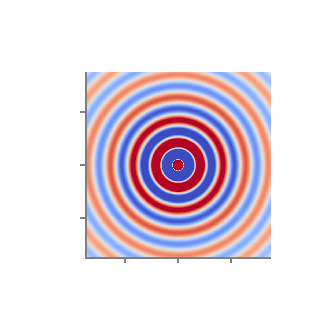
\includegraphics{sound_field_point_source}}%
    \gplfronttext
  \end{picture}%
\endgroup

%    \caption{Sound pressure for a monochromatic point
%        source~\eqref{eq:S:ps} placed at $(0,0,0)$. Parameters: $f =
%        800$\,Hz.
%        \reproduce{\GITHUB/fig2_05}}
%\end{figure}
%
The source model for a point source is given by the three dimensional Green's
function as\cite[][(6.73)]{Williams1999}
%
\begin{equation}
    S(\x,\omega) = A(\omega) \frac{1}{4\PI}
    \frac{\E^{-\I\omegac|\x-\xs|}}{|\x-\xs|}
    \qc
    \eqlabel{S:ps}
\end{equation}
%
where $\xs$ describes the position of the point source.

Transformed to the temporal domain this becomes
%
\begin{equation}
    s(\x,t) = a(t) * \frac{1}{4\PI} \frac{1}{|\x-\xs|}
    \deltafunc{t - \frac{|\x-\xs|}{c}}
    \qp
    \eqlabel{s:ps}
\end{equation}
%

The expansion coefficients for spherical basis functions are given
as\cite[][(2.37)]{Ahrens2012}
%
\begin{equation}
    \breve{S}_n^m(\theta_\text{s},\phi_\text{s},r_\text{s},\omega) =
    -\I \omegac \, h_n^{(2)}\!\!\left(\omegac r_\text{s}\right)
    Y_n^{-m}(\theta_\text{s},\phi_\text{s}) \qc
    \label{eq:point_source_spherical}
\end{equation}
%
where $(\phi_\text{s},\theta_\text{s},r_\text{s})$ describes the position of the
point source.

The expansion coefficients for linear basis functions are given
as\cite[][(C.10)]{Ahrens2012}
%
\begin{equation}
    \breve{S}(k_x,y,\omega) =
    -\frac{\I}{4} \H{0}{2} \left( \sqrt{(\tfrac{\omega}{c})^2-k_x^2} \;
        |y-y_\text{s}| \right) \chi(-k_x,x_\text{s}) \qc
    \label{eq:point_source_linear}
\end{equation}
%
for $|k_x|<|\omegac|$ and with $(x_\text{s},y_\text{s})$ describing the position
of the point source.

%----%----%----%----%----%----%----%----%----%----%----%----%----%----%----%----
\paragraph{3D Dipole Source}
\label{sec:dipole_source_3D}
%
The source model for a three dimensional dipole source is given by the
directional derivative of the three dimensional Green's function with respect to
\(\ns\) defining the orientation of the dipole source.
%
\begin{equation}
  \begin{aligned}
  S(\x,\omega) &= A(\omega) 
  \left\langle
    \nabla_{\xs} \left( \frac{1}{4\PI} \frac{\E^{-\I\omegac|\x-\xs|}}{|\x-\xs|}
    \right), \ns
  \right\rangle \\
  &=
    A(\omega)
    \frac{1}{4\PI} 
    \left( \frac{1}{|\x-\xs|} + \I \omegac \right)
    \frac{\langle \x-\xs, \ns \rangle}{|\x-\xs|^2}
    \E^{-\I\omegac|\x-\xs|}
  \qp
  \end{aligned}
  \eqlabel{S:dps}
\end{equation}
%
%\begin{figure}
%  \centering
%  \ft
%  % GNUPLOT: LaTeX picture with Postscript
\begingroup
  \makeatletter
  \providecommand\color[2][]{%
    \GenericError{(gnuplot) \space\space\space\@spaces}{%
      Package color not loaded in conjunction with
      terminal option `colourtext'%
    }{See the gnuplot documentation for explanation.%
    }{Either use 'blacktext' in gnuplot or load the package
      color.sty in LaTeX.}%
    \renewcommand\color[2][]{}%
  }%
  \providecommand\includegraphics[2][]{%
    \GenericError{(gnuplot) \space\space\space\@spaces}{%
      Package graphicx or graphics not loaded%
    }{See the gnuplot documentation for explanation.%
    }{The gnuplot epslatex terminal needs graphicx.sty or graphics.sty.}%
    \renewcommand\includegraphics[2][]{}%
  }%
  \providecommand\rotatebox[2]{#2}%
  \@ifundefined{ifGPcolor}{%
    \newif\ifGPcolor
    \GPcolortrue
  }{}%
  \@ifundefined{ifGPblacktext}{%
    \newif\ifGPblacktext
    \GPblacktextfalse
  }{}%
  % define a \g@addto@macro without @ in the name:
  \let\gplgaddtomacro\g@addto@macro
  % define empty templates for all commands taking text:
  \gdef\gplbacktext{}%
  \gdef\gplfronttext{}%
  \makeatother
  \ifGPblacktext
    % no textcolor at all
    \def\colorrgb#1{}%
    \def\colorgray#1{}%
  \else
    % gray or color?
    \ifGPcolor
      \def\colorrgb#1{\color[rgb]{#1}}%
      \def\colorgray#1{\color[gray]{#1}}%
      \expandafter\def\csname LTw\endcsname{\color{white}}%
      \expandafter\def\csname LTb\endcsname{\color{black}}%
      \expandafter\def\csname LTa\endcsname{\color{black}}%
      \expandafter\def\csname LT0\endcsname{\color[rgb]{1,0,0}}%
      \expandafter\def\csname LT1\endcsname{\color[rgb]{0,1,0}}%
      \expandafter\def\csname LT2\endcsname{\color[rgb]{0,0,1}}%
      \expandafter\def\csname LT3\endcsname{\color[rgb]{1,0,1}}%
      \expandafter\def\csname LT4\endcsname{\color[rgb]{0,1,1}}%
      \expandafter\def\csname LT5\endcsname{\color[rgb]{1,1,0}}%
      \expandafter\def\csname LT6\endcsname{\color[rgb]{0,0,0}}%
      \expandafter\def\csname LT7\endcsname{\color[rgb]{1,0.3,0}}%
      \expandafter\def\csname LT8\endcsname{\color[rgb]{0.5,0.5,0.5}}%
    \else
      % gray
      \def\colorrgb#1{\color{black}}%
      \def\colorgray#1{\color[gray]{#1}}%
      \expandafter\def\csname LTw\endcsname{\color{white}}%
      \expandafter\def\csname LTb\endcsname{\color{black}}%
      \expandafter\def\csname LTa\endcsname{\color{black}}%
      \expandafter\def\csname LT0\endcsname{\color{black}}%
      \expandafter\def\csname LT1\endcsname{\color{black}}%
      \expandafter\def\csname LT2\endcsname{\color{black}}%
      \expandafter\def\csname LT3\endcsname{\color{black}}%
      \expandafter\def\csname LT4\endcsname{\color{black}}%
      \expandafter\def\csname LT5\endcsname{\color{black}}%
      \expandafter\def\csname LT6\endcsname{\color{black}}%
      \expandafter\def\csname LT7\endcsname{\color{black}}%
      \expandafter\def\csname LT8\endcsname{\color{black}}%
    \fi
  \fi
  \setlength{\unitlength}{0.0500bp}%
  \begin{picture}(2834.00,2834.00)%
    \gplgaddtomacro\gplbacktext{%
      \colorrgb{0.50,0.50,0.50}%
      \put(550,887){\makebox(0,0)[r]{\strut{}$-1$}}%
      \colorrgb{0.50,0.50,0.50}%
      \put(550,1395){\makebox(0,0)[r]{\strut{}$0$}}%
      \colorrgb{0.50,0.50,0.50}%
      \put(550,1902){\makebox(0,0)[r]{\strut{}$1$}}%
      \colorrgb{0.50,0.50,0.50}%
      \put(1043,350){\makebox(0,0){\strut{}$-1$}}%
      \colorrgb{0.50,0.50,0.50}%
      \put(1550,350){\makebox(0,0){\strut{}$0$}}%
      \colorrgb{0.50,0.50,0.50}%
      \put(2057,350){\makebox(0,0){\strut{}$1$}}%
      \csname LTb\endcsname%
      \put(176,1394){\rotatebox{-270}{\makebox(0,0){\strut{}$y$ / m}}}%
      \put(1550,130){\makebox(0,0){\strut{}$x$ / m}}%
    }%
    \gplgaddtomacro\gplfronttext{%
    }%
    \gplbacktext
    \put(0,0){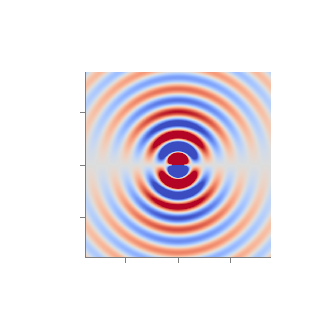
\includegraphics{sound_field_dipole_source}}%
    \gplfronttext
  \end{picture}%
\endgroup

%  \caption{Sound pressure for a monochromatic 3D dipole source
%    ~(\ref{eq:S:dps}) placed at $(0,0,0)$. Parameters: $f =
%    800$\,Hz.
%    \reproduce{\GITHUB/fig2_06}}
%\end{figure}
%
Transformed to the temporal domain this becomes
%
\begin{equation}
  s(\x,t) = a(t) *
  \left( \frac{1}{|\x-\xs|} + \IFT{ \frac{\I\omega}{c} } \right)
  *
  \frac{\langle \x-\xs, \ns \rangle}{4\PI |\x-\xs|^2}
  \deltafunc{t - \frac{|\x-\xs|}{c}} .
  \eqlabel{s:dps}
\end{equation}
%

%----%----%----%----%----%----%----%----%----%----%----%----%----%----%----%----
\paragraph{Line Source}
\label{sec:line_source}
%
The source model for a line source is given by the two dimensional Green's
function as\cite[][(8.47)]{Williams1999}
%
\begin{equation}
    S(\x,\omega) = -A(\omega) \frac{\I}{4} \H{0}{2} \left(\omegac |\x-\xs|\right)
    \qp
    \eqlabel{S:ls}
\end{equation}
%
%\begin{figure}
%    \centering
%    \ft
%    % GNUPLOT: LaTeX picture with Postscript
\begingroup
  \makeatletter
  \providecommand\color[2][]{%
    \GenericError{(gnuplot) \space\space\space\@spaces}{%
      Package color not loaded in conjunction with
      terminal option `colourtext'%
    }{See the gnuplot documentation for explanation.%
    }{Either use 'blacktext' in gnuplot or load the package
      color.sty in LaTeX.}%
    \renewcommand\color[2][]{}%
  }%
  \providecommand\includegraphics[2][]{%
    \GenericError{(gnuplot) \space\space\space\@spaces}{%
      Package graphicx or graphics not loaded%
    }{See the gnuplot documentation for explanation.%
    }{The gnuplot epslatex terminal needs graphicx.sty or graphics.sty.}%
    \renewcommand\includegraphics[2][]{}%
  }%
  \providecommand\rotatebox[2]{#2}%
  \@ifundefined{ifGPcolor}{%
    \newif\ifGPcolor
    \GPcolortrue
  }{}%
  \@ifundefined{ifGPblacktext}{%
    \newif\ifGPblacktext
    \GPblacktextfalse
  }{}%
  % define a \g@addto@macro without @ in the name:
  \let\gplgaddtomacro\g@addto@macro
  % define empty templates for all commands taking text:
  \gdef\gplbacktext{}%
  \gdef\gplfronttext{}%
  \makeatother
  \ifGPblacktext
    % no textcolor at all
    \def\colorrgb#1{}%
    \def\colorgray#1{}%
  \else
    % gray or color?
    \ifGPcolor
      \def\colorrgb#1{\color[rgb]{#1}}%
      \def\colorgray#1{\color[gray]{#1}}%
      \expandafter\def\csname LTw\endcsname{\color{white}}%
      \expandafter\def\csname LTb\endcsname{\color{black}}%
      \expandafter\def\csname LTa\endcsname{\color{black}}%
      \expandafter\def\csname LT0\endcsname{\color[rgb]{1,0,0}}%
      \expandafter\def\csname LT1\endcsname{\color[rgb]{0,1,0}}%
      \expandafter\def\csname LT2\endcsname{\color[rgb]{0,0,1}}%
      \expandafter\def\csname LT3\endcsname{\color[rgb]{1,0,1}}%
      \expandafter\def\csname LT4\endcsname{\color[rgb]{0,1,1}}%
      \expandafter\def\csname LT5\endcsname{\color[rgb]{1,1,0}}%
      \expandafter\def\csname LT6\endcsname{\color[rgb]{0,0,0}}%
      \expandafter\def\csname LT7\endcsname{\color[rgb]{1,0.3,0}}%
      \expandafter\def\csname LT8\endcsname{\color[rgb]{0.5,0.5,0.5}}%
    \else
      % gray
      \def\colorrgb#1{\color{black}}%
      \def\colorgray#1{\color[gray]{#1}}%
      \expandafter\def\csname LTw\endcsname{\color{white}}%
      \expandafter\def\csname LTb\endcsname{\color{black}}%
      \expandafter\def\csname LTa\endcsname{\color{black}}%
      \expandafter\def\csname LT0\endcsname{\color{black}}%
      \expandafter\def\csname LT1\endcsname{\color{black}}%
      \expandafter\def\csname LT2\endcsname{\color{black}}%
      \expandafter\def\csname LT3\endcsname{\color{black}}%
      \expandafter\def\csname LT4\endcsname{\color{black}}%
      \expandafter\def\csname LT5\endcsname{\color{black}}%
      \expandafter\def\csname LT6\endcsname{\color{black}}%
      \expandafter\def\csname LT7\endcsname{\color{black}}%
      \expandafter\def\csname LT8\endcsname{\color{black}}%
    \fi
  \fi
    \setlength{\unitlength}{0.0500bp}%
    \ifx\gptboxheight\undefined%
      \newlength{\gptboxheight}%
      \newlength{\gptboxwidth}%
      \newsavebox{\gptboxtext}%
    \fi%
    \setlength{\fboxrule}{0.5pt}%
    \setlength{\fboxsep}{1pt}%
\begin{picture}(2834.00,2834.00)%
    \gplgaddtomacro\gplbacktext{%
      \colorrgb{0.50,0.50,0.50}%
      \put(550,887){\makebox(0,0)[r]{\strut{}$-1$}}%
      \colorrgb{0.50,0.50,0.50}%
      \put(550,1395){\makebox(0,0)[r]{\strut{}$0$}}%
      \colorrgb{0.50,0.50,0.50}%
      \put(550,1902){\makebox(0,0)[r]{\strut{}$1$}}%
      \colorrgb{0.50,0.50,0.50}%
      \put(1043,350){\makebox(0,0){\strut{}$-1$}}%
      \colorrgb{0.50,0.50,0.50}%
      \put(1550,350){\makebox(0,0){\strut{}$0$}}%
      \colorrgb{0.50,0.50,0.50}%
      \put(2057,350){\makebox(0,0){\strut{}$1$}}%
    }%
    \gplgaddtomacro\gplfronttext{%
      \csname LTb\endcsname%
      \put(176,1394){\rotatebox{-270}{\makebox(0,0){\strut{}$y$ / m}}}%
      \put(1550,130){\makebox(0,0){\strut{}$x$ / m}}%
    }%
    \gplbacktext
    \put(0,0){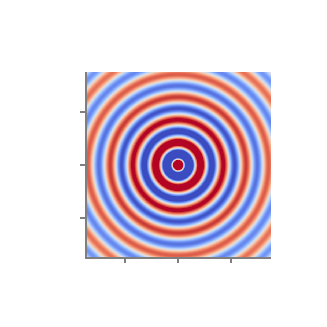
\includegraphics{sound_field_line_source}}%
    \gplfronttext
  \end{picture}%
\endgroup

%    \caption{Sound pressure for a monochromatic line
%    source~(\ref{eq:S:ls}) placed at $(0,0,0)$. Parameters: $f =
%        800$\,Hz.
%        \reproduce{\GITHUB/fig2_07}}
%\end{figure}
%
Applying the large argument approximation of the Hankel
function\cite[][(4.23)]{Williams1999} and transformed to
the temporal domain this becomes
%
\begin{equation}
    s(\x,t) = a(t) * \IFT{\sqrt{\frac{c}{\I\omega}}} * \sqrt{\frac{1}{8\PI}} \frac{1}{\sqrt{|\x-\xs|}}
    \deltafunc{t - \frac{|\x-\xs|}{c}}
    \qp
    \eqlabel{s:ls}
\end{equation}
%

The expansion coefficients for circular basis functions are given as
%
\begin{equation}
    \breve{S}_m(\phi_\text{s},r_\text{s},\omega) = -\frac{\I}{4}
    \H{m}{2} \left(\omegac r_\text{s}\right)
    \Phi_{-m}(\phi_\text{s}) \qp
    \label{eq:line_source_circular}
\end{equation}
%

The expansion coefficients for linear basis functions are given as
%
\begin{equation}
    \breve{S}(k_x,y_\text{s},\omega) = -\frac{\I}{2} \frac{1}{\sqrt{(\omegac)^2-k_x^2}}
    \chi(k_y,y_\text{s})\qp
    \label{eq:line_source_linear}
\end{equation}
%

%%%%%%%%%%%%%%%%%%%%%%%%%%%%%%%%%%%%%%%%%%%%%%%%%%%%%%%%%%%%%%%%%%%%%%%%%%%%%%%%%
\section{Driving Functions}
\label{sec:driving_functions}

In the following, driving functions for Near-Field Compensated High\-er Order
Ambisonics, the Spectral Division Method and Wave Field Synthesis are derived
for spherical, circular, and linear secondary source distributions. Among the
possible combinations of methods and secondary sources not all are
meaningful. Hence, only the relevant ones will be presented. The same holds for the
introduced source models of plane waves, point sources, line sources and focused
sources.
Ahrens and
Spors\cite{Ahrens2010a}
in addition have considered Spectral Division Method driving functions for
planar secondary source distributions.

The driving functions are given in the temporal-frequency domain. For some of them,
especially in the case of \ac{WFS} an analytic solution in the temporal
domain exists and is presented. For \ac{NFC-HOA}, temporal-domain implementations
for the \twohalfD cases are available for a plane wave and a point source as source models. The
derivation of the implementation is not explicitly shown here, but is described
in Spors et al.\cite{Spors2011b}

The \twohalfD cases are illustrated in the following by companion
figures, because only those cases will be investigated in the remainder of this
thesis.

%--%--%--%--%--%--%--%--%--%--%--%--%--%--%--%--%--%--%--%--%--%--%--%--%--%--%-
\subsection{Near-Field Compensated Higher Order Ambisonics and Spectral Division Method}
\label{sec:driving_functions_hoa}


%----%----%----%----%----%----%----%----%----%----%----%----%----%----%----%----
\paragraph{Plane Wave}
%
For a spherical secondary source distribution with radius $R_0$ the spherical
expansion coefficients of a
plane wave~\eqref{eq:plane_wave_spherical} and of the Green's
function for a point source~\eqref{eq:G_spherical} are inserted
into~\eqref{eq:D_spherical} and yield\cite[][(96)]{Schultz2014}
%
\begin{equation}
    D_\text{spherical}(\theta_0,\phi_0,\omega) = -A(\omega) \frac{4\PI}{R_0^{\,2}}
    \sum_{n=0}^\infty \sum_{m=-n}^n \frac{\I^{-n} Y_n^{-m}(\theta_k,\phi_k)}{\I\omegac h_n^{(2)}
    \left(\omegac R_0\right)} Y_n^m(\theta_0,\phi_0) \qp
    \eqlabel{D:hoa:pw:3D}
\end{equation}
%
%\begin{figure}
%    \centering
%    \ft
%    % GNUPLOT: LaTeX picture with Postscript
\begingroup
  \makeatletter
  \providecommand\color[2][]{%
    \GenericError{(gnuplot) \space\space\space\@spaces}{%
      Package color not loaded in conjunction with
      terminal option `colourtext'%
    }{See the gnuplot documentation for explanation.%
    }{Either use 'blacktext' in gnuplot or load the package
      color.sty in LaTeX.}%
    \renewcommand\color[2][]{}%
  }%
  \providecommand\includegraphics[2][]{%
    \GenericError{(gnuplot) \space\space\space\@spaces}{%
      Package graphicx or graphics not loaded%
    }{See the gnuplot documentation for explanation.%
    }{The gnuplot epslatex terminal needs graphicx.sty or graphics.sty.}%
    \renewcommand\includegraphics[2][]{}%
  }%
  \providecommand\rotatebox[2]{#2}%
  \@ifundefined{ifGPcolor}{%
    \newif\ifGPcolor
    \GPcolortrue
  }{}%
  \@ifundefined{ifGPblacktext}{%
    \newif\ifGPblacktext
    \GPblacktextfalse
  }{}%
  % define a \g@addto@macro without @ in the name:
  \let\gplgaddtomacro\g@addto@macro
  % define empty templates for all commands taking text:
  \gdef\gplbacktext{}%
  \gdef\gplfronttext{}%
  \makeatother
  \ifGPblacktext
    % no textcolor at all
    \def\colorrgb#1{}%
    \def\colorgray#1{}%
  \else
    % gray or color?
    \ifGPcolor
      \def\colorrgb#1{\color[rgb]{#1}}%
      \def\colorgray#1{\color[gray]{#1}}%
      \expandafter\def\csname LTw\endcsname{\color{white}}%
      \expandafter\def\csname LTb\endcsname{\color{black}}%
      \expandafter\def\csname LTa\endcsname{\color{black}}%
      \expandafter\def\csname LT0\endcsname{\color[rgb]{1,0,0}}%
      \expandafter\def\csname LT1\endcsname{\color[rgb]{0,1,0}}%
      \expandafter\def\csname LT2\endcsname{\color[rgb]{0,0,1}}%
      \expandafter\def\csname LT3\endcsname{\color[rgb]{1,0,1}}%
      \expandafter\def\csname LT4\endcsname{\color[rgb]{0,1,1}}%
      \expandafter\def\csname LT5\endcsname{\color[rgb]{1,1,0}}%
      \expandafter\def\csname LT6\endcsname{\color[rgb]{0,0,0}}%
      \expandafter\def\csname LT7\endcsname{\color[rgb]{1,0.3,0}}%
      \expandafter\def\csname LT8\endcsname{\color[rgb]{0.5,0.5,0.5}}%
    \else
      % gray
      \def\colorrgb#1{\color{black}}%
      \def\colorgray#1{\color[gray]{#1}}%
      \expandafter\def\csname LTw\endcsname{\color{white}}%
      \expandafter\def\csname LTb\endcsname{\color{black}}%
      \expandafter\def\csname LTa\endcsname{\color{black}}%
      \expandafter\def\csname LT0\endcsname{\color{black}}%
      \expandafter\def\csname LT1\endcsname{\color{black}}%
      \expandafter\def\csname LT2\endcsname{\color{black}}%
      \expandafter\def\csname LT3\endcsname{\color{black}}%
      \expandafter\def\csname LT4\endcsname{\color{black}}%
      \expandafter\def\csname LT5\endcsname{\color{black}}%
      \expandafter\def\csname LT6\endcsname{\color{black}}%
      \expandafter\def\csname LT7\endcsname{\color{black}}%
      \expandafter\def\csname LT8\endcsname{\color{black}}%
    \fi
  \fi
  \setlength{\unitlength}{0.0500bp}%
  \begin{picture}(2834.00,2834.00)%
    \gplgaddtomacro\gplbacktext{%
      \colorrgb{0.50,0.50,0.50}%
      \put(550,887){\makebox(0,0)[r]{\strut{}$-1$}}%
      \colorrgb{0.50,0.50,0.50}%
      \put(550,1395){\makebox(0,0)[r]{\strut{}$0$}}%
      \colorrgb{0.50,0.50,0.50}%
      \put(550,1902){\makebox(0,0)[r]{\strut{}$1$}}%
      \colorrgb{0.50,0.50,0.50}%
      \put(1043,350){\makebox(0,0){\strut{}$-1$}}%
      \colorrgb{0.50,0.50,0.50}%
      \put(1550,350){\makebox(0,0){\strut{}$0$}}%
      \colorrgb{0.50,0.50,0.50}%
      \put(2057,350){\makebox(0,0){\strut{}$1$}}%
      \csname LTb\endcsname%
      \put(176,1394){\rotatebox{-270}{\makebox(0,0){\strut{}$y$ / m}}}%
      \put(1550,130){\makebox(0,0){\strut{}$x$ / m}}%
    }%
    \gplgaddtomacro\gplfronttext{%
    }%
    \gplbacktext
    \put(0,0){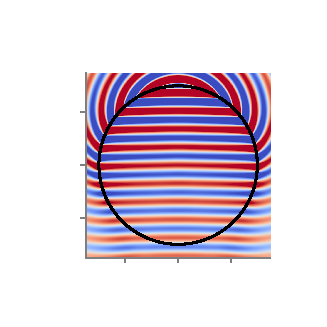
\includegraphics{sound_field_nfchoa_pw}}%
    \gplfronttext
  \end{picture}%
\endgroup

%    \caption{Sound pressure of a monochromatic plane wave synthesized with
%        \twohalfD \ac{NFC-HOA}~(\ref{eq:D:hoa:pw:2.5D}). Parameters: $\n_k = (0,-1,0)$,
%        $\xref = (0,0,0)$, $f = 1$\,kHz.
%        \reproduce{\GITHUB/fig2_08}}
%\end{figure}
%
For a circular secondary source distribution with radius $R_0$ the circular
expansion coefficients of a plane wave~\eqref{eq:plane_wave_circular} and
of the Green's function for a line source~\eqref{eq:G_circular} are
inserted into~\eqref{eq:D_circular} and
yield\cite[Compare][(16)]{Ahrens2009c}
%
\begin{equation}
    D_\text{circular}(\phi_0,\omega) = -A(\omega) \frac{2\I}{\PI R_0}
    \sum_{m=-\infty}^\infty \frac{\I^{-m}\Phi_{-m}(\phi_k)}
    {\H{m}{2}(\omegac R_0)} \Phi_m(\phi_0) \qp
    \eqlabel{D:hoa:pw:2D}
\end{equation}
%

For a circular secondary source distribution with radius $R_0$ and point source
as Green's function the \twohalfD driving function is given by inserting the
spherical expansion coefficients for a plane wave~\eqref{eq:plane_wave_spherical}
and a point source~\eqref{eq:point_source_spherical} into~\eqref{eq:D_circular_25D} as
%
\begin{equation}
    D_{\text{circular},\,\twohalfD}(\phi_0,\omega) = -A(\omega) \frac{2}{R_0}
    \sum_{m=-\infty}^\infty \frac{\I^{-|m|} \Phi_{-m}(\phi_k)} {\I\omegac
    h_{|m|}^{(2)}\left(\omegac R_0\right)} \Phi_m(\phi_0) \qp
    \eqlabel{D:hoa:pw:2.5D}
\end{equation}
%
For an infinite linear secondary source distribution located on the $x$-axis the
\twohalfD driving function is given by inserting the linear expansion coefficients
for a point source as Green's function~\eqref{eq:G_linear} and
a plane wave~\eqref{eq:plane_wave_linear} into~\eqref{eq:D_linear_25D} and
exploiting the fact that $(\frac{\omega}{c})^2 - k_{x_\text{s}}$ is constant. Assuming
$0 \le |k_{x_\text{s}}| \le |\omegac|$ this results
in\cite[][(17)]{Ahrens2010a}
%
\begin{equation}
    D_{\text{linear},\,\twohalfD}(x_0,\omega) = A(\omega) \frac{4\I
    \chi(k_y,y_\text{ref})}
    {\H{0}{2}(k_y y_\text{ref})} \chi(k_x,x_0) \qp
    \eqlabel{D:sdm:pw:2.5D}
\end{equation}
%

Transfered to the temporal domain this results
in\cite[][(18)]{Ahrens2010a}
%
\begin{equation}
    d_{\text{linear},\,\twohalfD}(x_0,t) = h(t) *
    a(t-\frac{x_0}{c}\sin\phi_k-\frac{y_\text{ref}}{c}\sin\phi_k)
    \qc
    \label{eq:d_sdm_pw_25D}
\end{equation}
%
where $\phi_k$ denotes the azimuth direction of the plane wave and
\begin{equation}
    h(t) =
    \IFT{\frac{4\I}{\H{0}{2}(k_y y_\text{ref})}} \qp
\end{equation}
The advantage of this
result is that it can be implemented by a simple weighting and delaying of
the signal, plus one convolution with $h(t)$. The same holds for the driving
functions of \ac{WFS} as presented in the next section.


%----%----%----%----%----%----%----%----%----%----%----%----%----%----%----%----
\paragraph{Point Source}
%
For a spherical secondary source distribution with radius $R_0$ the spherical
coefficients of a point source~\eqref{eq:point_source_spherical} and of the Green's
function~\eqref{eq:G_spherical} are inserted into~\eqref{eq:D_spherical} and yield
%
\begin{multline}
    D_\text{spherical}(\theta_0,\phi_0,\omega) = \\
    A(\omega) \frac{1}{R_0^{\,2}} \sum_{n=0}^\infty \sum_{m=-n}^n
    \frac{h_n^{(2)}(\omegac r_\text{s}) Y_n^{-m}(\theta_\text{s},\phi_\text{s})}
    {h_n^{(2)}(\omegac R_0)} Y_n^m (\theta_0,\phi_0) \qp
    \eqlabel{D:hoa:ps:3D}
\end{multline}
%
%\begin{figure}
%    \centering
%    \ft
%    % GNUPLOT: LaTeX picture with Postscript
\begingroup
  \makeatletter
  \providecommand\color[2][]{%
    \GenericError{(gnuplot) \space\space\space\@spaces}{%
      Package color not loaded in conjunction with
      terminal option `colourtext'%
    }{See the gnuplot documentation for explanation.%
    }{Either use 'blacktext' in gnuplot or load the package
      color.sty in LaTeX.}%
    \renewcommand\color[2][]{}%
  }%
  \providecommand\includegraphics[2][]{%
    \GenericError{(gnuplot) \space\space\space\@spaces}{%
      Package graphicx or graphics not loaded%
    }{See the gnuplot documentation for explanation.%
    }{The gnuplot epslatex terminal needs graphicx.sty or graphics.sty.}%
    \renewcommand\includegraphics[2][]{}%
  }%
  \providecommand\rotatebox[2]{#2}%
  \@ifundefined{ifGPcolor}{%
    \newif\ifGPcolor
    \GPcolortrue
  }{}%
  \@ifundefined{ifGPblacktext}{%
    \newif\ifGPblacktext
    \GPblacktextfalse
  }{}%
  % define a \g@addto@macro without @ in the name:
  \let\gplgaddtomacro\g@addto@macro
  % define empty templates for all commands taking text:
  \gdef\gplbacktext{}%
  \gdef\gplfronttext{}%
  \makeatother
  \ifGPblacktext
    % no textcolor at all
    \def\colorrgb#1{}%
    \def\colorgray#1{}%
  \else
    % gray or color?
    \ifGPcolor
      \def\colorrgb#1{\color[rgb]{#1}}%
      \def\colorgray#1{\color[gray]{#1}}%
      \expandafter\def\csname LTw\endcsname{\color{white}}%
      \expandafter\def\csname LTb\endcsname{\color{black}}%
      \expandafter\def\csname LTa\endcsname{\color{black}}%
      \expandafter\def\csname LT0\endcsname{\color[rgb]{1,0,0}}%
      \expandafter\def\csname LT1\endcsname{\color[rgb]{0,1,0}}%
      \expandafter\def\csname LT2\endcsname{\color[rgb]{0,0,1}}%
      \expandafter\def\csname LT3\endcsname{\color[rgb]{1,0,1}}%
      \expandafter\def\csname LT4\endcsname{\color[rgb]{0,1,1}}%
      \expandafter\def\csname LT5\endcsname{\color[rgb]{1,1,0}}%
      \expandafter\def\csname LT6\endcsname{\color[rgb]{0,0,0}}%
      \expandafter\def\csname LT7\endcsname{\color[rgb]{1,0.3,0}}%
      \expandafter\def\csname LT8\endcsname{\color[rgb]{0.5,0.5,0.5}}%
    \else
      % gray
      \def\colorrgb#1{\color{black}}%
      \def\colorgray#1{\color[gray]{#1}}%
      \expandafter\def\csname LTw\endcsname{\color{white}}%
      \expandafter\def\csname LTb\endcsname{\color{black}}%
      \expandafter\def\csname LTa\endcsname{\color{black}}%
      \expandafter\def\csname LT0\endcsname{\color{black}}%
      \expandafter\def\csname LT1\endcsname{\color{black}}%
      \expandafter\def\csname LT2\endcsname{\color{black}}%
      \expandafter\def\csname LT3\endcsname{\color{black}}%
      \expandafter\def\csname LT4\endcsname{\color{black}}%
      \expandafter\def\csname LT5\endcsname{\color{black}}%
      \expandafter\def\csname LT6\endcsname{\color{black}}%
      \expandafter\def\csname LT7\endcsname{\color{black}}%
      \expandafter\def\csname LT8\endcsname{\color{black}}%
    \fi
  \fi
    \setlength{\unitlength}{0.0500bp}%
    \ifx\gptboxheight\undefined%
      \newlength{\gptboxheight}%
      \newlength{\gptboxwidth}%
      \newsavebox{\gptboxtext}%
    \fi%
    \setlength{\fboxrule}{0.5pt}%
    \setlength{\fboxsep}{1pt}%
\begin{picture}(2834.00,2834.00)%
    \gplgaddtomacro\gplbacktext{%
      \colorrgb{0.50,0.50,0.50}%
      \put(550,887){\makebox(0,0)[r]{\strut{}$-1$}}%
      \colorrgb{0.50,0.50,0.50}%
      \put(550,1395){\makebox(0,0)[r]{\strut{}$0$}}%
      \colorrgb{0.50,0.50,0.50}%
      \put(550,1902){\makebox(0,0)[r]{\strut{}$1$}}%
      \colorrgb{0.50,0.50,0.50}%
      \put(1043,350){\makebox(0,0){\strut{}$-1$}}%
      \colorrgb{0.50,0.50,0.50}%
      \put(1550,350){\makebox(0,0){\strut{}$0$}}%
      \colorrgb{0.50,0.50,0.50}%
      \put(2057,350){\makebox(0,0){\strut{}$1$}}%
    }%
    \gplgaddtomacro\gplfronttext{%
      \csname LTb\endcsname%
      \put(176,1394){\rotatebox{-270}{\makebox(0,0){\strut{}$y$ / m}}}%
      \put(1550,130){\makebox(0,0){\strut{}$x$ / m}}%
    }%
    \gplbacktext
    \put(0,0){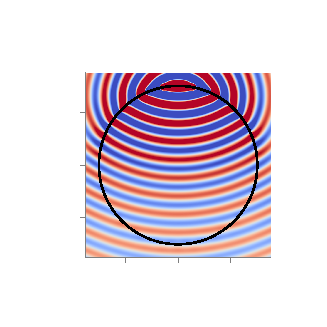
\includegraphics{sound_field_nfchoa_ps}}%
    \gplfronttext
  \end{picture}%
\endgroup

%    \caption{Sound pressure for a monochromatic point source synthesized by
%        \twohalfD \ac{NFC-HOA}~\eqref{eq:D:hoa:ps:2.5D}. Parameters: $\xs =
%        (0,2.5,0)$\,m, $\xref = (0,0,0)$, $f = 1$\,kHz.
%        \reproduce{\GITHUB/fig2_09}}
%\end{figure}
%
For a circular secondary source distribution with radius $R_0$ and point source
as secondary sources the \twohalfD driving function is given by inserting the
spherical coefficients~\eqref{eq:point_source_spherical} and~\eqref{eq:G_spherical}
into~\eqref{eq:D_circular_25D} as
%
\begin{equation}
    D_{\text{circular},\,\twohalfD}(\phi_0,\omega) = A(\omega) \frac{1}{2\PI R_0}
        \sum_{m=-\infty}^{\infty}
        \frac{h_{|m|}^{(2)} (\omegac r_s) \Phi_{-m}(\phi_\text{s})} 
        {h_{|m|}^{(2)} (\omegac R_0)} \Phi_m(\phi_0) \qp
    \eqlabel{D:hoa:ps:2.5D}
\end{equation}
%

For an infinite linear secondary source distribution located on the $x$-axis and
point sources as secondary sources the \twohalfD driving function for a
point source is given by inserting the corresponding linear expansion
coefficients~\eqref{eq:point_source_linear} and~\eqref{eq:G_linear}
into~\eqref{eq:D_linear_25D}. Assuming
$0 \le |k_x| < |\omegac|$ this results
in\cite[Compare (4.53) in][]{Ahrens2012}
%
\begin{multline}
    D_{\text{linear},\,\twohalfD}(x_0,\omega) = \\
    A(\omega) \int_{-\infty}^\infty \frac{
    \H{0}{2}\left(\sqrt{(\omegac)^2-k_x^2} \; (y_\text{ref}-y_\text{s}) \right)
    \chi(-k_x,x_\text{s})} {\H{0}{2}\left(\sqrt{(\omegac)^2-k_x^2} \;
    y_\text{ref}\right)} \chi(k_x,x_0) \, \D{k_x} \qp
    \eqlabel{D:sdm:ps:2.5D}
\end{multline}
%


%----%----%----%----%----%----%----%----%----%----%----%----%----%----%----%----
\paragraph{Line Source}
%
For a circular secondary source distribution with radius $R_0$ and line sources
as secondary sources the driving function is given by inserting the
circular coefficients~\eqref{eq:line_source_circular} and~\eqref{eq:G_circular}
into~\eqref{eq:D_circular} as
%
\begin{equation}
    D_{\text{circular}}(\phi_0,\omega) = A(\omega) \frac{1}{2\PI R_0}
        \sum_{m=-\infty}^{\infty}
        \frac{\H{m}{2}(\omegac r_s) \Phi_{-m}(\phi_\text{s})}
        {\H{m}{2}(\omegac R_0)} \Phi_m(\phi_0) \qp
    \label{eq:D_nfchoa_ls_2D}
\end{equation}
%

For an infinite linear secondary source distribution located on the $x$-axis and
line sources as secondary sources the driving function is given by inserting the
linear coefficients~\eqref{eq:line_source_linear} and~\eqref{eq:G_circular}
into~\eqref{eq:D_linear} as
%
\begin{equation}
    D_\text{linear}(x_0,\omega) = A(\omega) \frac{1}{2\PI}
    \int_{-\infty}^\infty \chi(k_y,y_s) \chi(k_x,x_0) \, \D{k_x} \qp
\end{equation}
%


%----%----%----%----%----%----%----%----%----%----%----%----%----%----%----%----
\paragraph{Focused Source}
%
Focused sources mimic point or line sources that are located inside the audience
area. For the single-layer potential the assumption is that the audience area is
free from sources and sinks. However, a focused source is neither of them. It
represents a sound field that converges towards a focal point and diverges
afterwards. This can be achieved by reversing the driving function of a point or
line source in time which is known as time reversal
focusing.\cite{Yon2003}

Nonetheless, the single-layer potential should not be solved for focused sources
without any approximation. In the near field of a source,
evanescent
waves\cite[][p.\,24]{Williams1999} appear for spatial frequencies $k_x > |\omegac|$.
They decay exponentially with the distance from the source. An exact solution for a focused
source is supposed to include these evanescent waves around the focal point.
That is only
possible by applying very large amplitudes to the secondary
sources.\cite[Compare Fig.\,2a in][]{Spors2010}
Since the evanescent waves decay rapidly and are hence not
influencing the perception, they can easily be omitted.
For corresponding driving functions for focused sources without the
evanescent part of the sound field see Spors and
Ahrens\cite{Spors2010} for
\ac{SDM} and Ahrens and Spors\cite{Ahrens2009d} for \ac{NFC-HOA}.

In this thesis only focused sources in \ac{WFS} will be considered.


%--%--%--%--%--%--%--%--%--%--%--%--%--%--%--%--%--%--%--%--%--%--%--%--%--%--%-
\subsection{Wave Field Synthesis}
\label{sec:driving_functions_wfs}

In the following, the driving functions for \ac{WFS} in the frequency and
temporal domain
for selected source models are presented. The temporal domain
functions consist of a filtering of the source signal and a weighting and
delaying of the individual secondary source signals. This property allows for a very efficient
implementation of \ac{WFS} driving functions in the temporal domain.
It is one of the main advantages of \ac{WFS} in comparison
to most of the \ac{NFC-HOA}/\ac{SDM} solutions discussed above.

%----%----%----%----%----%----%----%----%----%----%----%----%----%----%----%----
\paragraph{Plane Wave}
%
By inserting the source model of a plane wave~\eqref{eq:S:pw}
into~\eqref{eq:D_wfs} and~\eqref{eq:D25D_wfs} it follows
%
\begin{equation}
    D(\x_0,\omega) = 2 w(\x_0) A(\omega) \I\omegac \n_k\n_{\x_0}
    \E^{-\I\omegac\n_k\x_0} \qc
    \eqlabel{D:wfs:pw}
\end{equation}
%
\begin{equation}
    D_\twohalfD(\x_0,\omega) = 2g_0 w(\x_0) A(\omega) \sqrt{\I\omegac} \n_k\n_{\x_0} 
    \E^{-\I\omegac\n_k\x_0} \qp
    \eqlabel{D:wfs:pw:2.5D}
\end{equation}
%
%\begin{figure}[-0.5cm]
%    \centering
%    \ft
%    % GNUPLOT: LaTeX picture with Postscript
\begingroup
  \makeatletter
  \providecommand\color[2][]{%
    \GenericError{(gnuplot) \space\space\space\@spaces}{%
      Package color not loaded in conjunction with
      terminal option `colourtext'%
    }{See the gnuplot documentation for explanation.%
    }{Either use 'blacktext' in gnuplot or load the package
      color.sty in LaTeX.}%
    \renewcommand\color[2][]{}%
  }%
  \providecommand\includegraphics[2][]{%
    \GenericError{(gnuplot) \space\space\space\@spaces}{%
      Package graphicx or graphics not loaded%
    }{See the gnuplot documentation for explanation.%
    }{The gnuplot epslatex terminal needs graphicx.sty or graphics.sty.}%
    \renewcommand\includegraphics[2][]{}%
  }%
  \providecommand\rotatebox[2]{#2}%
  \@ifundefined{ifGPcolor}{%
    \newif\ifGPcolor
    \GPcolortrue
  }{}%
  \@ifundefined{ifGPblacktext}{%
    \newif\ifGPblacktext
    \GPblacktextfalse
  }{}%
  % define a \g@addto@macro without @ in the name:
  \let\gplgaddtomacro\g@addto@macro
  % define empty templates for all commands taking text:
  \gdef\gplbacktext{}%
  \gdef\gplfronttext{}%
  \makeatother
  \ifGPblacktext
    % no textcolor at all
    \def\colorrgb#1{}%
    \def\colorgray#1{}%
  \else
    % gray or color?
    \ifGPcolor
      \def\colorrgb#1{\color[rgb]{#1}}%
      \def\colorgray#1{\color[gray]{#1}}%
      \expandafter\def\csname LTw\endcsname{\color{white}}%
      \expandafter\def\csname LTb\endcsname{\color{black}}%
      \expandafter\def\csname LTa\endcsname{\color{black}}%
      \expandafter\def\csname LT0\endcsname{\color[rgb]{1,0,0}}%
      \expandafter\def\csname LT1\endcsname{\color[rgb]{0,1,0}}%
      \expandafter\def\csname LT2\endcsname{\color[rgb]{0,0,1}}%
      \expandafter\def\csname LT3\endcsname{\color[rgb]{1,0,1}}%
      \expandafter\def\csname LT4\endcsname{\color[rgb]{0,1,1}}%
      \expandafter\def\csname LT5\endcsname{\color[rgb]{1,1,0}}%
      \expandafter\def\csname LT6\endcsname{\color[rgb]{0,0,0}}%
      \expandafter\def\csname LT7\endcsname{\color[rgb]{1,0.3,0}}%
      \expandafter\def\csname LT8\endcsname{\color[rgb]{0.5,0.5,0.5}}%
    \else
      % gray
      \def\colorrgb#1{\color{black}}%
      \def\colorgray#1{\color[gray]{#1}}%
      \expandafter\def\csname LTw\endcsname{\color{white}}%
      \expandafter\def\csname LTb\endcsname{\color{black}}%
      \expandafter\def\csname LTa\endcsname{\color{black}}%
      \expandafter\def\csname LT0\endcsname{\color{black}}%
      \expandafter\def\csname LT1\endcsname{\color{black}}%
      \expandafter\def\csname LT2\endcsname{\color{black}}%
      \expandafter\def\csname LT3\endcsname{\color{black}}%
      \expandafter\def\csname LT4\endcsname{\color{black}}%
      \expandafter\def\csname LT5\endcsname{\color{black}}%
      \expandafter\def\csname LT6\endcsname{\color{black}}%
      \expandafter\def\csname LT7\endcsname{\color{black}}%
      \expandafter\def\csname LT8\endcsname{\color{black}}%
    \fi
  \fi
  \setlength{\unitlength}{0.0500bp}%
  \begin{picture}(2834.00,2834.00)%
    \gplgaddtomacro\gplbacktext{%
      \colorrgb{0.50,0.50,0.50}%
      \put(550,887){\makebox(0,0)[r]{\strut{}$-1$}}%
      \colorrgb{0.50,0.50,0.50}%
      \put(550,1395){\makebox(0,0)[r]{\strut{}$0$}}%
      \colorrgb{0.50,0.50,0.50}%
      \put(550,1902){\makebox(0,0)[r]{\strut{}$1$}}%
      \colorrgb{0.50,0.50,0.50}%
      \put(1043,350){\makebox(0,0){\strut{}$-1$}}%
      \colorrgb{0.50,0.50,0.50}%
      \put(1550,350){\makebox(0,0){\strut{}$0$}}%
      \colorrgb{0.50,0.50,0.50}%
      \put(2057,350){\makebox(0,0){\strut{}$1$}}%
      \csname LTb\endcsname%
      \put(176,1394){\rotatebox{-270}{\makebox(0,0){\strut{}$y$ / m}}}%
      \put(1550,130){\makebox(0,0){\strut{}$x$ / m}}%
    }%
    \gplgaddtomacro\gplfronttext{%
    }%
    \gplbacktext
    \put(0,0){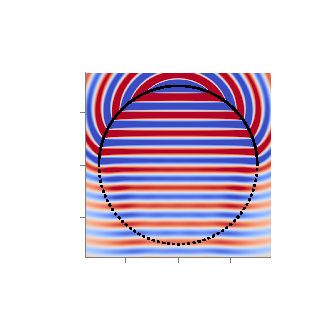
\includegraphics{sound_field_wfs_pw}}%
    \gplfronttext
  \end{picture}%
\endgroup

%    \caption{Sound pressure for a monochromatic plane wave synthesized by
%    \twohalfD \ac{WFS}~(\ref{eq:D:wfs:pw:2.5D}). Parameters: $\n_k = (0,-1,0)$, $\xref
%        = (0,0,0)$, $f = 1$\,kHz.
%        \reproduce{\GITHUB/fig2_10}}
%\end{figure}
%
Transfered to the temporal domain via an inverse Fourier
transform~\eqref{eq:ift}, it follows
%
\begin{equation}
    d(\x_0,t) = 2 a(t) * h(t) * w(\x_0) \n_k \n_{\x_0} \deltafunc{t -
    \frac{\n_k\x_0}{c}} \qc
    \eqlabel{d:wfs:pw}
\end{equation}
%
\begin{equation}
    d_\twohalfD(\x_0,t) = 2g_0 a(t) * h_\twohalfD(t) * w(\x_0) \n_k \n_{\x_0}
    \deltafunc{t - \frac{\n_k\x_0}{c}} \qc
    \eqlabel{d:wfs:pw:2.5D}
\end{equation}
%
where
\begin{equation}
    h(t) = \IFT{\I\omegac} \qc
    \eqlabel{wfs:preeq}
\end{equation}
and
\begin{equation}
    h_\twohalfD(t) = \IFT{\sqrt{\I\omegac}}
    \eqlabel{wfs:preeq:2.5D}
\end{equation}
denote the so called pre-equalization filters in \ac{WFS}.

The window function $w(\x_0)$ for a plane wave as source model can be
calculated after Spors et al. as\cite{Spors2008}
%
\begin{equation}
    w(\x_0) = 
    \begin{cases}
        1 & \n_k \n_{\x_0} > 0 \\
        0 & \text{else}
    \end{cases}
    \eqlabel{wfs:pw:selection}
\end{equation}
%



%----%----%----%----%----%----%----%----%----%----%----%----%----%----%----%----
\paragraph{Point Source}
%
By inserting the source model for a point
source~\eqref{eq:S:ps}
into~\eqref{eq:D_wfs} and~\eqref{eq:D25D_wfs} it follows
%
%\begin{figure}
%    \centering
%    \ft
%    % GNUPLOT: LaTeX picture with Postscript
\begingroup
  \makeatletter
  \providecommand\color[2][]{%
    \GenericError{(gnuplot) \space\space\space\@spaces}{%
      Package color not loaded in conjunction with
      terminal option `colourtext'%
    }{See the gnuplot documentation for explanation.%
    }{Either use 'blacktext' in gnuplot or load the package
      color.sty in LaTeX.}%
    \renewcommand\color[2][]{}%
  }%
  \providecommand\includegraphics[2][]{%
    \GenericError{(gnuplot) \space\space\space\@spaces}{%
      Package graphicx or graphics not loaded%
    }{See the gnuplot documentation for explanation.%
    }{The gnuplot epslatex terminal needs graphicx.sty or graphics.sty.}%
    \renewcommand\includegraphics[2][]{}%
  }%
  \providecommand\rotatebox[2]{#2}%
  \@ifundefined{ifGPcolor}{%
    \newif\ifGPcolor
    \GPcolortrue
  }{}%
  \@ifundefined{ifGPblacktext}{%
    \newif\ifGPblacktext
    \GPblacktextfalse
  }{}%
  % define a \g@addto@macro without @ in the name:
  \let\gplgaddtomacro\g@addto@macro
  % define empty templates for all commands taking text:
  \gdef\gplbacktext{}%
  \gdef\gplfronttext{}%
  \makeatother
  \ifGPblacktext
    % no textcolor at all
    \def\colorrgb#1{}%
    \def\colorgray#1{}%
  \else
    % gray or color?
    \ifGPcolor
      \def\colorrgb#1{\color[rgb]{#1}}%
      \def\colorgray#1{\color[gray]{#1}}%
      \expandafter\def\csname LTw\endcsname{\color{white}}%
      \expandafter\def\csname LTb\endcsname{\color{black}}%
      \expandafter\def\csname LTa\endcsname{\color{black}}%
      \expandafter\def\csname LT0\endcsname{\color[rgb]{1,0,0}}%
      \expandafter\def\csname LT1\endcsname{\color[rgb]{0,1,0}}%
      \expandafter\def\csname LT2\endcsname{\color[rgb]{0,0,1}}%
      \expandafter\def\csname LT3\endcsname{\color[rgb]{1,0,1}}%
      \expandafter\def\csname LT4\endcsname{\color[rgb]{0,1,1}}%
      \expandafter\def\csname LT5\endcsname{\color[rgb]{1,1,0}}%
      \expandafter\def\csname LT6\endcsname{\color[rgb]{0,0,0}}%
      \expandafter\def\csname LT7\endcsname{\color[rgb]{1,0.3,0}}%
      \expandafter\def\csname LT8\endcsname{\color[rgb]{0.5,0.5,0.5}}%
    \else
      % gray
      \def\colorrgb#1{\color{black}}%
      \def\colorgray#1{\color[gray]{#1}}%
      \expandafter\def\csname LTw\endcsname{\color{white}}%
      \expandafter\def\csname LTb\endcsname{\color{black}}%
      \expandafter\def\csname LTa\endcsname{\color{black}}%
      \expandafter\def\csname LT0\endcsname{\color{black}}%
      \expandafter\def\csname LT1\endcsname{\color{black}}%
      \expandafter\def\csname LT2\endcsname{\color{black}}%
      \expandafter\def\csname LT3\endcsname{\color{black}}%
      \expandafter\def\csname LT4\endcsname{\color{black}}%
      \expandafter\def\csname LT5\endcsname{\color{black}}%
      \expandafter\def\csname LT6\endcsname{\color{black}}%
      \expandafter\def\csname LT7\endcsname{\color{black}}%
      \expandafter\def\csname LT8\endcsname{\color{black}}%
    \fi
  \fi
  \setlength{\unitlength}{0.0500bp}%
  \begin{picture}(2834.00,2834.00)%
    \gplgaddtomacro\gplbacktext{%
      \colorrgb{0.50,0.50,0.50}%
      \put(550,887){\makebox(0,0)[r]{\strut{}$-1$}}%
      \colorrgb{0.50,0.50,0.50}%
      \put(550,1395){\makebox(0,0)[r]{\strut{}$0$}}%
      \colorrgb{0.50,0.50,0.50}%
      \put(550,1902){\makebox(0,0)[r]{\strut{}$1$}}%
      \colorrgb{0.50,0.50,0.50}%
      \put(1043,350){\makebox(0,0){\strut{}$-1$}}%
      \colorrgb{0.50,0.50,0.50}%
      \put(1550,350){\makebox(0,0){\strut{}$0$}}%
      \colorrgb{0.50,0.50,0.50}%
      \put(2057,350){\makebox(0,0){\strut{}$1$}}%
      \csname LTb\endcsname%
      \put(176,1394){\rotatebox{-270}{\makebox(0,0){\strut{}$y$ / m}}}%
      \put(1550,130){\makebox(0,0){\strut{}$x$ / m}}%
    }%
    \gplgaddtomacro\gplfronttext{%
    }%
    \gplbacktext
    \put(0,0){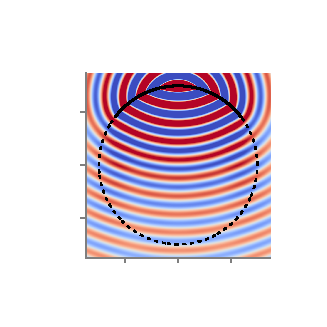
\includegraphics{sound_field_wfs_ps}}%
    \gplfronttext
  \end{picture}%
\endgroup

%    \caption{Sound pressure for a monochromatic point source synthesized by
%        \twohalfD \ac{WFS}~(\ref{eq:D:wfs:ps:2.5D}). Parameters: $\xs = (0,2.5,0)$\,m,
%        $\xref = (0,0,0)$, $f = 1$\,kHz.
%        \reproduce{\GITHUB/fig2_11}}
%\end{figure}
%
\begin{multline}
    D(\x_0,\omega) = \\
    \frac{1}{2\PI} A(\omega) w(\x_0) \left(\I\omegac +
    \frac{1}{|\x_0-\xs|} \right) \frac{(\x_0-\xs)\n_{\x_0}}{|\x_0-\xs|^2}
    \E^{-\I\omegac |\x_0-\xs|} \qc
    \eqlabel{D:wfs:ps:woapprox}
\end{multline}
%
\begin{multline}
    D_\twohalfD(\x_0,\omega) = \\
    \frac{g_0}{2\PI} A(\omega) w(\x_0) \sqrt{\I\omegac} \left(
    1 + \frac{1}{\I\omegac|\x_0-\xs|}
    \right) \frac{(\x_0-\xs) \n_{\x_0}}{|\x_0-\xs|^2} \E^{-\I\omegac |\x_0-\xs|} \qp
    \eqlabel{D:wfs:ps:woapprox:2.5D}
\end{multline}
%
Under the assumption of $|\x_0-\xs| \gg
1$~\eqref{eq:D:wfs:ps:woapprox}
and~\eqref{eq:D:wfs:ps:woapprox:2.5D} can be approximated by
%
\begin{equation}
    D(\x_0,\omega) = \frac{1}{2\PI} A(\omega) w(\x_0) \I\omegac
    \frac{(\x_0-\xs)\n_{\x_0}}{|\x_0-\xs|^{\nicefrac{3}{2}}}
    \E^{-\I\omegac |\x_0-\xs|} \qc
    \eqlabel{D:wfs:ps}
\end{equation}
%
\begin{multline}
    D_\twohalfD(\x_0,\omega) = \\
    \frac{g_0}{2\PI} A(\omega) w(\x_0) \sqrt{\I\omegac}
    \frac{(\x_0-\xs)\n_{\x_0}}{|\x_0-\xs|^{\nicefrac{3}{2}}}
    \E^{-\I\omegac |\x_0-\xs|} \qc
    \eqlabel{D:wfs:ps:2.5D}
\end{multline}
%
which is the traditional formulation of a point source in
\ac{WFS} as given for the \twohalfD case in
Verheijen.\cite[][(2.22a), whereby $r$ corresponds to $|\x_0-\xs|$ and
$\cos\varphi$ to $\frac{(\x_0-\xs)\n_{\x_0}}{|\x_0-\xs|}$]{Verheijen1997}
It has the advantage that its temporal domain version could again be implemented as
a simple weighting- and delaying-mechanism.
This is the default driving function for a point source in the Sound Field
Synthesis Toolbox.

Transfered to the temporal domain via an inverse Fourier transform~\eqref{eq:ift} it follows
%
\begin{equation}
    d(\x_0,t) = \frac{1}{2\PI} a(t) * h(t) * w(\x_0)
    \frac{(\x_0-\xs)\n_{\x_0}}{|\x_0-\xs|^{\nicefrac{3}{2}}}
    \deltafunc{t-\frac{|\x_0-\xs|}{c}} \qc
    \eqlabel{d:wfs:ps}
\end{equation}
%
\begin{multline}
    d_\twohalfD(\x_0,t) = \\
    \frac{g_0}{2\PI} a(t) * h_\twohalfD(t) * w(\x_0)
    \frac{(\x_0-\xs)\n_{\x_0}}{|\x_0-\xs|^{\nicefrac{3}{2}}}
    \deltafunc{t-\frac{|\x_0-\xs|}{c}} \qp
    \eqlabel{d:wfs:ps:2.5D}
\end{multline}
%
The window function $w(\x_0)$ for a point source as source model can be
calculated after Spors at al. as\cite{Spors2008}
%
\begin{equation}
    w(\x_0) = 
    \begin{cases}
        1 & (\x_0-\xs) \n_{\x_0} > 0 \\
        0 & \text{else}
    \end{cases}
    \eqlabel{wfs:ps:selection}
\end{equation}
%


%----%----%----%----%----%----%----%----%----%----%----%----%----%----%----%----
\paragraph{Line Source}
%
By inserting the source model for a line source~\eqref{eq:S:ls}
into~\eqref{eq:D_wfs} and~\eqref{eq:D25D_wfs} and calculating the derivate of
the Hankel function\cite[][(9.1.30)]{Abramowitz1972} it follows
%
\begin{equation}
    D(\x_0,\omega) = -\frac{1}{2}A(\omega) w(\x_0) \I\omegac
    \frac{(\x_0-\xs)\n_{\x_0}}{|\x_0-\xs|}
    \H{1}{2}\left(\omegac|\x_0-\xs|\right) \qc
    \eqlabel{D:wfs:ls}
\end{equation}
%
\begin{multline}
    D_\twohalfD(\x_0,\omega) = \\
    -\frac{1}{2}g_0 A(\omega) w(\x_0) \sqrt{\I\omegac}
    \frac{(\x_0-\xs)\n_{\x_0}}{|\x_0-\xs|}
    \H{1}{2}\left(\omegac|\x_0-\xs|\right) \qp
    \eqlabel{D:wfs:ls:2.5D}
\end{multline}
%
%\begin{figure}
%    \centering
%    \ft
%    % GNUPLOT: LaTeX picture with Postscript
\begingroup
  \makeatletter
  \providecommand\color[2][]{%
    \GenericError{(gnuplot) \space\space\space\@spaces}{%
      Package color not loaded in conjunction with
      terminal option `colourtext'%
    }{See the gnuplot documentation for explanation.%
    }{Either use 'blacktext' in gnuplot or load the package
      color.sty in LaTeX.}%
    \renewcommand\color[2][]{}%
  }%
  \providecommand\includegraphics[2][]{%
    \GenericError{(gnuplot) \space\space\space\@spaces}{%
      Package graphicx or graphics not loaded%
    }{See the gnuplot documentation for explanation.%
    }{The gnuplot epslatex terminal needs graphicx.sty or graphics.sty.}%
    \renewcommand\includegraphics[2][]{}%
  }%
  \providecommand\rotatebox[2]{#2}%
  \@ifundefined{ifGPcolor}{%
    \newif\ifGPcolor
    \GPcolortrue
  }{}%
  \@ifundefined{ifGPblacktext}{%
    \newif\ifGPblacktext
    \GPblacktextfalse
  }{}%
  % define a \g@addto@macro without @ in the name:
  \let\gplgaddtomacro\g@addto@macro
  % define empty templates for all commands taking text:
  \gdef\gplbacktext{}%
  \gdef\gplfronttext{}%
  \makeatother
  \ifGPblacktext
    % no textcolor at all
    \def\colorrgb#1{}%
    \def\colorgray#1{}%
  \else
    % gray or color?
    \ifGPcolor
      \def\colorrgb#1{\color[rgb]{#1}}%
      \def\colorgray#1{\color[gray]{#1}}%
      \expandafter\def\csname LTw\endcsname{\color{white}}%
      \expandafter\def\csname LTb\endcsname{\color{black}}%
      \expandafter\def\csname LTa\endcsname{\color{black}}%
      \expandafter\def\csname LT0\endcsname{\color[rgb]{1,0,0}}%
      \expandafter\def\csname LT1\endcsname{\color[rgb]{0,1,0}}%
      \expandafter\def\csname LT2\endcsname{\color[rgb]{0,0,1}}%
      \expandafter\def\csname LT3\endcsname{\color[rgb]{1,0,1}}%
      \expandafter\def\csname LT4\endcsname{\color[rgb]{0,1,1}}%
      \expandafter\def\csname LT5\endcsname{\color[rgb]{1,1,0}}%
      \expandafter\def\csname LT6\endcsname{\color[rgb]{0,0,0}}%
      \expandafter\def\csname LT7\endcsname{\color[rgb]{1,0.3,0}}%
      \expandafter\def\csname LT8\endcsname{\color[rgb]{0.5,0.5,0.5}}%
    \else
      % gray
      \def\colorrgb#1{\color{black}}%
      \def\colorgray#1{\color[gray]{#1}}%
      \expandafter\def\csname LTw\endcsname{\color{white}}%
      \expandafter\def\csname LTb\endcsname{\color{black}}%
      \expandafter\def\csname LTa\endcsname{\color{black}}%
      \expandafter\def\csname LT0\endcsname{\color{black}}%
      \expandafter\def\csname LT1\endcsname{\color{black}}%
      \expandafter\def\csname LT2\endcsname{\color{black}}%
      \expandafter\def\csname LT3\endcsname{\color{black}}%
      \expandafter\def\csname LT4\endcsname{\color{black}}%
      \expandafter\def\csname LT5\endcsname{\color{black}}%
      \expandafter\def\csname LT6\endcsname{\color{black}}%
      \expandafter\def\csname LT7\endcsname{\color{black}}%
      \expandafter\def\csname LT8\endcsname{\color{black}}%
    \fi
  \fi
  \setlength{\unitlength}{0.0500bp}%
  \begin{picture}(2834.00,2834.00)%
    \gplgaddtomacro\gplbacktext{%
      \colorrgb{0.50,0.50,0.50}%
      \put(550,887){\makebox(0,0)[r]{\strut{}$-1$}}%
      \colorrgb{0.50,0.50,0.50}%
      \put(550,1395){\makebox(0,0)[r]{\strut{}$0$}}%
      \colorrgb{0.50,0.50,0.50}%
      \put(550,1902){\makebox(0,0)[r]{\strut{}$1$}}%
      \colorrgb{0.50,0.50,0.50}%
      \put(1043,350){\makebox(0,0){\strut{}$-1$}}%
      \colorrgb{0.50,0.50,0.50}%
      \put(1550,350){\makebox(0,0){\strut{}$0$}}%
      \colorrgb{0.50,0.50,0.50}%
      \put(2057,350){\makebox(0,0){\strut{}$1$}}%
      \csname LTb\endcsname%
      \put(176,1394){\rotatebox{-270}{\makebox(0,0){\strut{}$y$ / m}}}%
      \put(1550,130){\makebox(0,0){\strut{}$x$ / m}}%
    }%
    \gplgaddtomacro\gplfronttext{%
    }%
    \gplbacktext
    \put(0,0){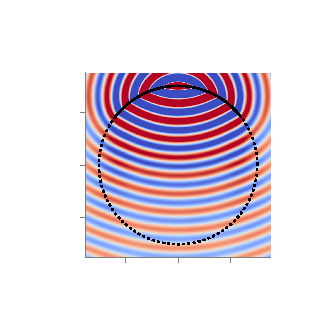
\includegraphics{sound_field_wfs_ls}}%
    \gplfronttext
  \end{picture}%
\endgroup

%    \caption{Sound pressure for a monochromatic line source synthesized by
%        \twohalfD \ac{WFS}~\eqref{eq:D:wfs:ls:2.5D}. Parameters: $\xs = (0,2.5,0)$\,m,
%        $\xref = (0,0,0)$, $f = 1$\,kHz.
%        \reproduce{\GITHUB/fig2_12}}
%\end{figure}
%
Applying $\H{1}{2}(\zeta) \approx -\sqrt{\frac{2}{\PI \I\zeta}} \E^{-\I\zeta}$ for $z\gg1$ after
Williams\cite[][(4.23)]{Williams1999} and transfered to the
temporal domain via an inverse Fourier
transform~\eqref{eq:ift} it follows
%
\begin{equation}
    d(\x_0,t) = \sqrt{\frac{1}{2\PI}} a(t) * h(t) *
    w(\x0) \frac{(\x_0-\xs)\n_{\x_0}}{|\x_0-\xs|^{\nicefrac{3}{2}}}
    \deltafunc{t-\frac{|\x_0-\xs|}{c}} \qc
    \eqlabel{d:wfs:ls}
\end{equation}
%
\begin{multline}
    d_\twohalfD(\x_0,t) = \\
    g_0 \sqrt{\frac{1}{2\PI}} a(t) *
    \IFT{\sqrt{\frac{c}{\I\omega}}} * w(\x0)
    \frac{(\x_0-\xs)\n_{\x_0}}{|\x_0-\xs|^{\nicefrac{3}{2}}}
    \deltafunc{t-\frac{|\x_0-\xs|}{c}} \qp
    \label{eq:d:wfs:ls_25D}
\end{multline}
%
The window function $w(\x_0)$ for a line source as source model can be
calculated after Spors et al. as\cite{Spors2008}
%
\begin{equation}
    w(\x_0) = 
    \begin{cases}
        1 & (\x_0-\xs) \n_{\x_0} > 0 \\
        0 & \text{else}
    \end{cases}
    \eqlabel{wfs:ls:selection}
\end{equation}
%



%----%----%----%----%----%----%----%----%----%----%----%----%----%----%----%----
\paragraph{Focused Source}
%
%\begin{figure}
%    \centering
%    \ft
%    % GNUPLOT: LaTeX picture with Postscript
\begingroup
  \makeatletter
  \providecommand\color[2][]{%
    \GenericError{(gnuplot) \space\space\space\@spaces}{%
      Package color not loaded in conjunction with
      terminal option `colourtext'%
    }{See the gnuplot documentation for explanation.%
    }{Either use 'blacktext' in gnuplot or load the package
      color.sty in LaTeX.}%
    \renewcommand\color[2][]{}%
  }%
  \providecommand\includegraphics[2][]{%
    \GenericError{(gnuplot) \space\space\space\@spaces}{%
      Package graphicx or graphics not loaded%
    }{See the gnuplot documentation for explanation.%
    }{The gnuplot epslatex terminal needs graphicx.sty or graphics.sty.}%
    \renewcommand\includegraphics[2][]{}%
  }%
  \providecommand\rotatebox[2]{#2}%
  \@ifundefined{ifGPcolor}{%
    \newif\ifGPcolor
    \GPcolortrue
  }{}%
  \@ifundefined{ifGPblacktext}{%
    \newif\ifGPblacktext
    \GPblacktextfalse
  }{}%
  % define a \g@addto@macro without @ in the name:
  \let\gplgaddtomacro\g@addto@macro
  % define empty templates for all commands taking text:
  \gdef\gplbacktext{}%
  \gdef\gplfronttext{}%
  \makeatother
  \ifGPblacktext
    % no textcolor at all
    \def\colorrgb#1{}%
    \def\colorgray#1{}%
  \else
    % gray or color?
    \ifGPcolor
      \def\colorrgb#1{\color[rgb]{#1}}%
      \def\colorgray#1{\color[gray]{#1}}%
      \expandafter\def\csname LTw\endcsname{\color{white}}%
      \expandafter\def\csname LTb\endcsname{\color{black}}%
      \expandafter\def\csname LTa\endcsname{\color{black}}%
      \expandafter\def\csname LT0\endcsname{\color[rgb]{1,0,0}}%
      \expandafter\def\csname LT1\endcsname{\color[rgb]{0,1,0}}%
      \expandafter\def\csname LT2\endcsname{\color[rgb]{0,0,1}}%
      \expandafter\def\csname LT3\endcsname{\color[rgb]{1,0,1}}%
      \expandafter\def\csname LT4\endcsname{\color[rgb]{0,1,1}}%
      \expandafter\def\csname LT5\endcsname{\color[rgb]{1,1,0}}%
      \expandafter\def\csname LT6\endcsname{\color[rgb]{0,0,0}}%
      \expandafter\def\csname LT7\endcsname{\color[rgb]{1,0.3,0}}%
      \expandafter\def\csname LT8\endcsname{\color[rgb]{0.5,0.5,0.5}}%
    \else
      % gray
      \def\colorrgb#1{\color{black}}%
      \def\colorgray#1{\color[gray]{#1}}%
      \expandafter\def\csname LTw\endcsname{\color{white}}%
      \expandafter\def\csname LTb\endcsname{\color{black}}%
      \expandafter\def\csname LTa\endcsname{\color{black}}%
      \expandafter\def\csname LT0\endcsname{\color{black}}%
      \expandafter\def\csname LT1\endcsname{\color{black}}%
      \expandafter\def\csname LT2\endcsname{\color{black}}%
      \expandafter\def\csname LT3\endcsname{\color{black}}%
      \expandafter\def\csname LT4\endcsname{\color{black}}%
      \expandafter\def\csname LT5\endcsname{\color{black}}%
      \expandafter\def\csname LT6\endcsname{\color{black}}%
      \expandafter\def\csname LT7\endcsname{\color{black}}%
      \expandafter\def\csname LT8\endcsname{\color{black}}%
    \fi
  \fi
    \setlength{\unitlength}{0.0500bp}%
    \ifx\gptboxheight\undefined%
      \newlength{\gptboxheight}%
      \newlength{\gptboxwidth}%
      \newsavebox{\gptboxtext}%
    \fi%
    \setlength{\fboxrule}{0.5pt}%
    \setlength{\fboxsep}{1pt}%
\begin{picture}(2834.00,2834.00)%
    \gplgaddtomacro\gplbacktext{%
      \colorrgb{0.50,0.50,0.50}%
      \put(550,887){\makebox(0,0)[r]{\strut{}$-1$}}%
      \colorrgb{0.50,0.50,0.50}%
      \put(550,1395){\makebox(0,0)[r]{\strut{}$0$}}%
      \colorrgb{0.50,0.50,0.50}%
      \put(550,1902){\makebox(0,0)[r]{\strut{}$1$}}%
      \colorrgb{0.50,0.50,0.50}%
      \put(1043,350){\makebox(0,0){\strut{}$-1$}}%
      \colorrgb{0.50,0.50,0.50}%
      \put(1550,350){\makebox(0,0){\strut{}$0$}}%
      \colorrgb{0.50,0.50,0.50}%
      \put(2057,350){\makebox(0,0){\strut{}$1$}}%
    }%
    \gplgaddtomacro\gplfronttext{%
      \csname LTb\endcsname%
      \put(176,1394){\rotatebox{-270}{\makebox(0,0){\strut{}$y$ / m}}}%
      \put(1550,130){\makebox(0,0){\strut{}$x$ / m}}%
    }%
    \gplbacktext
    \put(0,0){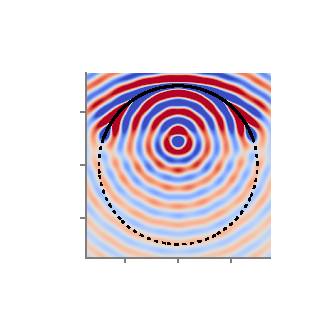
\includegraphics{sound_field_wfs_fs}}%
    \gplfronttext
  \end{picture}%
\endgroup

%    \caption{Sound pressure of a mono-frequent focused source synthesized with
%        \twohalfD \ac{WFS}~(\ref{eq:D:wfs:fs:2.5D}). Parameters: $\xs = (0,0.5,0)$\,m,
%        $\n_\text{s} = (0,-1,0)$, $\xref = (0,0,0)$, $f = 1$\,kHz.
%        \reproduce{\GITHUB/fig2_13}}
%    \label{fig:wfs_focused_source}
%\end{figure}
%
As mentioned before, focused sources exhibit a field that converges in a focal
point inside the audience area. After passing the focal
point, the field becomes a diverging one as can be seen in
Figure~\ref{fig:wfs_focused_source}. In order to choose the active secondary
sources, especially for circular or spherical geometries, the focused source
also needs a direction $\n_\text{s}$.

The driving function for a focused source are given by the time-reversed
versions of the driving functions for a point source as
%
\begin{multline}
    D(\x_0,\omega) = \\
    \frac{1}{2\PI} A(\omega) w(\x_0) \left(\I\omegac +
    \frac{1}{|\x_0-\xs|} \right) \frac{(\x_0-\xs)\n_{\x_0}}{|\x_0-\xs|^2}
    \E^{\I\omegac |\x_0-\xs|} \qc
    \eqlabel{D:wfs:fs:woapprox}
\end{multline}
%
\begin{multline}
    D_\twohalfD(\x_0,\omega) = \\
    \frac{g_0}{2\PI} A(\omega) w(\x_0) \sqrt{\I\omegac} \left(
    1 + \frac{1}{\I\omegac|\x_0-\xs|}
    \right) \frac{(\x_0-\xs) \n_{\x_0}}{|\x_0-\xs|^2} \E^{\I\omegac |\x_0-\xs|}
    \qc
    \eqlabel{D:wfs:fs:woapprox:2.5D}
\end{multline}
%
or by using an approximated point source as
%
\begin{equation}
    D(\x_0,\omega) = \frac{1}{2\PI} A(\omega) w(\x_0) \I\omegac
    \frac{(\x_0-\xs)\n_{\x_0}}{|\x_0-\xs|^{\nicefrac{3}{2}}}
    \E^{\I\omegac |\x_0-\xs|} \qc
    \eqlabel{D:wfs:fs}
\end{equation}
%
\begin{equation}
    D_\twohalfD(\x_0,\omega) = \frac{g_0}{2\PI} A(\omega) w(\x_0) \sqrt{\I\omegac}
    \frac{(\x_0-\xs)\n_{\x_0}}{|\x_0-\xs|^{\nicefrac{3}{2}}}
    \E^{\I\omegac |\x_0-\xs|} \qp
    \eqlabel{D:wfs:fs:2.5D}
\end{equation}
%
As before for other source types, the approximated versions are the default driving functions for a focused
source used in this thesis.

Transfered to the temporal domain via an inverse Fourier transform~\eqref{eq:ift} it follows
%
\begin{equation}
    d(\x_0,t) = \frac{1}{2\PI} a(t) * h(t) * w(\x_0)
    \frac{(\x_0-\xs)\n_{\x_0}}{|\x_0-\xs|^{\nicefrac{3}{2}}}
    \deltafunc{t+\frac{|\x_0-\xs|}{c}} \qc
    \eqlabel{d:wfs:fs}
\end{equation}
%
\begin{multline}
    d_\twohalfD(\x_0,t) = \\
    \frac{g_0}{2\PI} a(t) * h_\twohalfD(t) * w(\x_0)
    \frac{(\x_0-\xs)\n_{\x_0}}{|\x_0-\xs|^{\nicefrac{3}{2}}}
    \deltafunc{t+\frac{|\x_0-\xs|}{c}} \qp
    \eqlabel{d:wfs:fs:2.5D}
\end{multline}
%
In this thesis a focused source always refers to the time-reversed
version of a point source, but a focused line source can be defined in the
same way starting from~\eqref{eq:D:wfs:ls}
%
\begin{equation}
    D(\x_0,\omega) = -\frac{1}{2}A(\omega) w(\x_0) \I\omegac
    \frac{(\x_0-\xs)\n_{\x_0}}{|\x_0-\xs|}
    \H{1}{1}\left(\omegac|\x_0-\xs|\right) \qp
    \eqlabel{D:wfs:fs:ls}
\end{equation}
%
The window function $w(\x_0)$ for a focused source can be
calculated as
%
\begin{equation}
    w(\x_0) = 
    \begin{cases}
        1 & \n_\text{s} (\xs-\x_0) > 0 \\
        0 & \text{else}
    \end{cases}
    \eqlabel{wfs:fs:selection}
\end{equation}
%


%%%%%%%%%%%%%%%%%%%%%%%%%%%%%%%%%%%%%%%%%%%%%%%%%%%%%%%%%%%%%%%%%%%%%%%%%%%%%%%%

%--%--%--%--%--%--%--%--%--%--%--%--%--%--%--%--%--%--%--%--%--%--%--%--%--%--%-
\subsection{Local Sound Field Synthesis}
\label{sec:driving_functions_localwfs}

The reproduction accuracy of \ac{WFS} is limited due to practical aspects. For 
the 
audible frequency range the desired sound field can not be synthesized 
aliasing-free over an extended listening area, which is surrounded by a 
discrete ensemble of individually driven loudspeakers. However, it is suitable 
for certain applications to increase reproduction accuracy inside a smaller 
(local) listening region while stronger artifacts outside are permitted. The 
implemented Local Wave Field Synthesis method utilizes focused sources as a 
distribution of virtual loudspeakers which are placed more densely around the 
local listening area. These virtual loudspeakers can be driven by conventional 
\ac{SFS} techniques, like e.g. \ac{WFS} or \ac{NFC-HOA}. The results are 
similar to band-limited \ac{NFC-HOA}, with the difference that the form and 
position of the enhanced area can freely be chosen within the listening area.

The set of focused sources is treated as a virtual loudspeaker 
distribution and their positions \(\xfs\) are subsumed under 
\(\mathcal{X}_{\mathrm{fs}}\). Therefore, each focused source is driven 
individually by 
\(D_l(\xfs, \omega)\), which in principle can be any driving function for real 
loudspeakers mentioned in previous sections. At the moment however, only 
\ac{WFS} and \ac{NFC-HOA} driving functions are supported. The resulting 
driving function for a loudspeaker located at \(\x_0\) reads
%
\begin{equation}
  D(\x_0,\omega) = \sum_{\xfs \in \mathcal{X}_{\mathrm{fs}}} 
  D_{\mathrm l}(\xfs, \omega) 
  D_{\mathrm{fs}}(\x_0,\xfs,\omega) \qc
  \eqlabel{D:localwfs}
\end{equation}
%
which is superposition of the driving function 
\(D_{\mathrm l}{\mathrm{fs}}(\x_0,\xfs,\omega)\) reproducing a single 
focused source at \(\xfs\) weighted by \(D_l(\xfs, \omega)\). Former is 
derived by replacing \(\xs\) with 
\(\xfs\) in the WFS driving functions \eqref{eq:D:wfs:fs} and 
\eqref{eq:d:wfs:fs:2.5D} for focused sources. This yields
%
\begin{equation}
  D_{\mathrm{fs}}(\x_0,\xfs,\omega) =
    \frac{1}{2\PI} A(\omega) w(\x_0) \I\omegac
    \frac{(\x_0-\xfs)\n_{\x_0}}{|\x_0-\xfs|^{\nicefrac{3}{2}}}
    \E^{\I\omegac |\x_0-\xfs|}
\end{equation}
%
and
%
\begin{equation}
  D_{\mathrm{fs,2.5D}}(\x_0,\xfs,\omega) = 
    \frac{g_0}{2\PI} A(\omega) w(\x_0) \sqrt{\I\omegac}
    \frac{(\x_0-\xs)\n_{\x_0}}{|\x_0-\xs|^{\nicefrac{3}{2}}}
    \E^{\I\omegac |\x_0-\xs|} \qp
\end{equation}
for the 2.5D case. For the temporal domain, inverse Fourier transform yields 
the driving signals
%
\begin{equation}
  d(\x_0,t) = \sum_{\xfs \in \mathcal{X}_{\mathrm{fs}}} 
    d_{\mathrm l}(\xfs, t) * d_{\mathrm{fs}}(\x_0,\xfs, t) \qc
  \eqlabel{d:localwfs}
\end{equation}
%
while \(d_{\mathrm{fs}}(\x_0,\xfs, t)\) is derived analogously to
\eqref{eq:D:localwfs} from \eqref{eq:d:wfs:fs} or \eqref{eq:d:wfs:fs:2.5D}. At 
the moment \(d_{\mathrm l}(\xfs, t)\) does only support driving functions from 
\ac{WFS}.
